\section{Group -- Zone HVAC Air Loop Terminal Units}\label{group-zone-HVAC-air-loop-terminal-units}

The systems described in the Air Distribution Units (ADU's) are shown below. A variety of air terminal units are available for connecting air systems to thermal zones. These single description ADU's contain the reference to the components and the actual controls in one block of input. The idea is that the control volume is drawn tightly around the controls and loosely around the components. This allows complex interactions to take place between all of the components that respond to the Zone Thermostatic Control output. The coils that are referenced in the ADU's are explained fully in the ``Coils'' section of this manual.

\subsection{AirTerminal:SingleDuct:ConstantVolume:Reheat}\label{airterminalsingleductconstantvolumereheat}

The AirTerminal:SingleDuct:ConstantVolume:Reheat or terminal reheat system is a constant volume reheat system. The systems cooling capabilities are provided by way of cooling coil that supplies cooling to the entire supply air volume. The cooling coil is controlled by a controller setpoint specified for the cooling coil. Zone control is accomplished by heating (reheating) the airflow into each zone as determined by the zone thermostat. Currently the reheat can be supplied by a electric, gas, or hot water coil that tries to meet the zone demand.

\subsubsection{Inputs}

\paragraph{Field: Name}

Unique name for the terminal reheat Air Distribution Unit (ADU).

\paragraph{Field: Availability Schedule Name}

Schedule that this component will operate or is available to operate. A schedule value greater than 0 (usually 1 is used) indicates that the component can be on during the time period. A value less than or equal to 0 (usually 0 is used) denotes that the component must be off for the time period. If this field is blank, the schedule has values of 1 for all time periods.

\paragraph{Field: Air Outlet Node Name}

The outlet node from the ADU to the zone. This is the same node as the reheat component air outlet node.

\paragraph{Field: Air Inlet Node Name}

The air-inlet node name that connects the air splitter to the individual zone ADU. This is the same node as the reheat component air inlet node.

\paragraph{Field: Maximum Air Flow Rate}

The design constant volume flow rate (m\(^{3}\)/sec) specified for the terminal reheat ADU.

\paragraph{Field: Reheat Coil Object Type}\label{field-reheat-coil-object-type}

The valid reheat component objects currently available are:

\begin{itemize}
\item
  \hyperref[coilheatingwater]{Coil:Heating:Water}
\item
  \hyperref[coilheatingelectric]{Coil:Heating:Electric}
\item
  \hyperref[coilheatinggas-000]{Coil:Heating:Fuel}
\item
  \hyperref[coilheatingsteam]{Coil:Heating:Steam}
\end{itemize}

\paragraph{Field: Reheat Coil Name}\label{field-reheat-coil-name}

Reheat Coil Object name being simulated with this ADU. Applicable for all coils.

\paragraph{Field: Maximum Hot Water or Steam Flow Rate}\label{field-maximum-hot-water-or-steam-flow-rate}

This field is zero for gas and electric coils. Set to the maximum design hot water or steam volumetric flow rate in m\(^{3}\)/s for the hot water or steam heating coil. The steam volumetric~ flow rate is calculated at 100C and 101325 Pa.

\paragraph{Field: Minimum Hot Water or Steam Flow Rate}\label{field-minimum-hot-water-or-steam-flow-rate}

This field is zero for gas and electric coils. Set to the minimum design hot water or steam volumetric flow rate in m\(^{3}\)/s for the hot water or steam coil, normally set to be a shut off valve that is set to zero. The steam volumetric~ flow rate is calculated at 100C and 101325 Pa.

\paragraph{Field: Convergence Tolerance}\label{field-convergence-tolerance}

The coil is controlled by knowing the zone demand determined by the zone thermostat and setting the outlet conditions to meet this demand. For the electric and gas coils, this is set exactly since the coil model solution can be inverted. With the hot water coil that uses an effectiveness-NTU method, the solution cannot be inverted directly. Therefore, to determine the correct mass flow rate for the hot water the solution is solved for by iteration. The iterative solution uses an interval halving routine and needs a termination criterion that is set with the Convergence Tolerance parameter. This control offset is set to a decimal fraction of the zone demand as the criteria, i.e.~0.001. The default for the field is 0.001.

\paragraph{Field: Maximum Reheat Air Temperature}\label{field-maximum-reheat-air-temperature}

This is the upper limit on the temperature in degrees C of the air leaving the terminal unit -- reheat coil (and being delivered to the zone). If the user leaves this field blank, no maximum reheat air temperature is enforced.

\subsubsection{Outputs}

\begin{itemize}
\item
  HVAC,Average,Zone Air Terminal Outdoor Air Volume Flow Rate {[}m3/s{]}
\end{itemize}

\paragraph{Zone Air Terminal Outdoor Air Volume Flow Rate {[}m3/s{]}}\label{zone-air-terminal-outdoor-air-volume-flow-rate-m3s}

This output is the amount of outdoor air entering the zone. This is the average value over the frequency being reported. The amount of outdoor air is defined as the terminal unit air volume flow rate multiplied by the fraction of outdoor air entering the air loop's outside air system.

An IDF example:

\begin{lstlisting}

AirTerminal:SingleDuct:ConstantVolume:Reheat,
      Reheat Zone 1,  !- Name of System
      FanAndCoilAvailSched,  !- Availability schedule for VAV System
      Zone 1 Reheat Air Outlet Node,  !- Unit Air Outlet Node
      Zone 1 Reheat Air Inlet Node,  !- Unit Air Inlet Node
      0.59,  !- Maximum air flow rate {m3/s}
      COIL:Gas:Heating,  !- Reheat Component Object
      Reheat Coil Zone 1,  !- Name of Reheat Component
      0.0,  !- Max Reheat Water Flow {m3/s}
      0.0,  !- Min Reheat Water Flow {m3/s}
      0.001;  !- Convergence Tolerance
\end{lstlisting}

\subsection{AirTerminal:SingleDuct:ConstantVolume:NoReheat}\label{airterminalsingleductconstantvolumenoreheat}
The AirTerminal:SingleDuct:ConstantVolume:NoReheat object creates the capability of supplying central system air directly to a zone without any zone level thermostat control. The supply air temperature is controlled by the central system controller. It is typically used with a unitary system and furnaces which controls the system supply temperature and flow rate with continuous or cycling fan. When used without the Design Specification Outdoor Air Object Name, the terminal unit is passive and accepts any flow rate supplied by the central system, but will never exceed the maximum air flow rate.

This object allows the program to know what zone this branch of the air system is attached to, and input fields for availability schedule, air inlet and outlet nodes, the maximum air flow rate, and other two optional input fields. The air inlet node should be the same as one of the \emph{\hyperref[airloophvaczonesplitter]{AirLoopHVAC:ZoneSplitter}} or \emph{\hyperref[airloophvacsupplyplenum]{AirLoopHVAC:SupplyPlenum}} component  outlet nodes. The air outlet node name should be same as zone air inlet node name and the air distribution unit air outlet node name. The last two optional input fields: \textit{Design Specification Outdoor Air Object Name}, and \textit{Per Person Ventilation Rate Mode} are used for modulating the outdoor air requirement of an air terminal unit depending on the method.

\subsubsection{Inputs}\label{inputs-1-001}

\paragraph{Field: Name}\label{field-name-1-000}

A unique user assigned name for the single duct constant volume no reheat air terminal unit.

\paragraph{Field: Availability Schedule Name}\label{field-availability-schedule-name-1}

Availability schedule name for this system. Schedule value > 0 means the system is available or else the system is off. If this field is blank, the system is always available.

\paragraph{Field: Air Inlet Node Name}\label{field-air-inlet-node-name}

The air inlet node name that connects the air splitter to the individual zone air distribution unit. This node should also be one of the outlet air node of an \hyperref[airloophvaczonesplitter]{AirLoopHVAC:ZoneSplitter} or \hyperref[airloophvacsupplyplenum]{AirLoopHVAC:SupplyPlenum} component.

\paragraph{Field: Air Outlet Node Name}\label{field-air-outlet-node-name}

This is an air outlet node from the air distribution unit. This node name should be one of the supply air inlet node names of the zone served by this component.

\paragraph{Field: Maximum Air Flow Rate}\label{field-maximum-air-flow-rate-1}

The design maximum volume flow rate~ (m\(^{3}\)/sec). This field is autosizable.

\paragraph{Field: Design Specification Outdoor Air Object Name}

This field is used to modulate the terminal unit flow rate based on the specified outdoor air requirement. When the name of a \hyperref[designspecificationoutdoorair]{DesignSpecification:OutdoorAir} or \hyperref[designspecificationoutdoorairspacelist]{DesignSpecification:OutdoorAir:SpaceList} object is entered, the terminal unit will adjust flow to meet this outdoor air requirement and no more. Load is still "Uncontrolled." If Outdoor Air Flow per Person is non-zero, then the outdoor air requirement will be computed based on either the current or design occupancy as specified in the \textit{Per Person Ventilation Rate Mode} input field below. At no time will the supply air flow rate exceed the value for Maximum Air Flow Rate. The requested flow rate may not be fully met if the system is operating with cycling fan. The volume flow rate is converted to mass flow rate using the standard density of air at Pressure = 101325 Pa, Temperature = 20C, and Humidity Ratio = 0.0. If this field is blank, then the terminal unit will not be controlled for outdoor air flow. This field is optional.

\paragraph{Field: Per Person Ventilation Rate Mode}\label{field-per-person-ventilation-rate-mode}

This field specifies the occupancy level to use when calculating the ventilation rate per person when a Design Specification Outdoor Air Object Name has been specified. \textit{CurrentOccupancy} uses the current number of people in the zone which may vary. \textit{DesignOccupancy} uses the total Number of People specified for the zone which is constant.

\subsubsection{Outputs}

\begin{itemize}
\item
  HVAC,Average,Zone Air Terminal Outdoor Air Volume Flow Rate {[}m3/s{]}
\end{itemize}

\paragraph{Zone Air Terminal Outdoor Air Volume Flow Rate {[}m3/s{]}}

This output is the amount of outdoor air entering the zone. This is the average value over the frequency being reported. The amount of outdoor air is defined as the terminal unit air volume flow rate multiplied by the fraction of outdoor air entering the air loop's outside air system.

An IDF example:

\begin{lstlisting}

AirTerminal:SingleDuct:ConstantVolume:NoReheat,
      NoReheat Zone 1,                !- Name of System
      AlwaysOnFanAvailSched,          !- Availability Schedule Name
      Zone 1 Unit Air Inlet Node,     !- Air Inlet Node Name
      Zone 1 Unit Air Outlet Node,    !- Air Outlet Node Name
      0.60,                           !- Maximum Air Flow Rate {m3/s}
      ,                               !- Design Specification Outdoor Air Object Name
      ;                               !- Per Person Ventilation Rate Mode
\end{lstlisting}

\subsection{AirTerminal:SingleDuct:VAV:Reheat}\label{airterminalsingleductvavreheat}

AirTerminal:SingleDuct:VAV:Reheat - Variable air volume (VAV) systems control the dry-bulb temperature inside a zone by varying the supply air volume instead of the air temperature. At full cooling the VAV damper is fully open supplying the specified maximum air flow rate. As the cooling load decreases, the damper closes until it reaches the minimum stop specified by the zone minimum air flow fraction. The zone minimum supply air flow can be further adjusted using scheduled fraction values specified in the field \textit{Minimum Air Flow Turndown Schedule Name}.

VAV systems can be used for interior or perimeter zones with a common fan system, air temperature control, and reheating devices. The VAV concept may vary according to the VAV box locations, air temperature controls and types of heating elements. Heating can usually be provided by use of reheat coils or thermostatic baseboard.

\subsubsection{Inputs}\label{inputs-2-001}

\paragraph{Field: Name}\label{field-name-2-000}

Unique name for the AirTerminal:SingleDuct:VAV:Reheat Air Distribution Unit (ADU).

\paragraph{Field: Availability Schedule Name}\label{field-availability-schedule-name-2}

Schedule that this component will operate or is available to operate. A schedule value greater than 0 (usually 1 is used) indicates that the component can be on during the time period. A value less than or equal to 0 (usually 0 is used) denotes that the component must be off for the time period. If this field is blank, the schedule has values of 1 for all time periods.

\paragraph{Field: Damper Air Outlet Node Name}\label{field-damper-air-outlet-node-name}

The VAV damper outlet node. This is the outlet node of the damper and the inlet node of the reheat coil.

\paragraph{Field: Air Inlet Node Name}\label{field-air-inlet-node-name-1}

The air inlet node name that connects the air splitter to the individual zone ADU. This is \emph{not} the same as the air inlet node of the reheat component: it is upstream of that node. This is the inlet node to the terminal unit and the damper

\paragraph{Field: Maximum Air Flow Rate}\label{field-maximum-air-flow-rate-2}

The design maximum volume flow rate (m\(^{3}\)/sec) specified for VAV ADU.

\paragraph{Field: Zone Minimum Air Flow Method}\label{field-zone-minimum-air-flow-method}

This field is used to select how the program will determine the minimum flow rate to the zone while the system is operating.~ The minimum flow rate is modeled as a fraction of the maximum flow rate.~ There are three choices for selecting how the minimum flow rate is specified:~ Constant, FixedFlowRate, and Scheduled.~ If Constant is entered, then the program will use the value for the constant minimum air flow fraction entered in the following field.~ If FixedFlowRate is entered, then the program will use the value for minimum flow rate entered in the field below called Fixed Minimum Air Flow Rate.~ If Scheduled is entered, then the program will obtain the value for minimum flow fraction from the schedule named in the field below called Minimum Air Flow Fraction Schedule Name.~ The default is Constant.

\paragraph{Field: Constant Minimum Air Flow Fraction}\label{field-constant-minimum-air-flow-fraction}

The minimum flow rate to the zone while the system is operating, specified as a fraction of the maximum air flow rate. The minimum zone fraction is normally specified to meet the minimum ventilation requirement for the occupants. The reheat coil operates only when the damper is at this minimum flow rate when Damper Heating Action is set to Normal.~ This field is used if the previous field is set to Constant.~ If the previous field is set to Scheduled (and the field Maximum Hot Water or Steam Flow Rate is set to autosize), then this field is optional and can be used to separately control the air flow rate used for sizing normal-action reheat coils. If this field and the following field have values, the greater of the two is used for sizing.

This field is autosizable and defaulted to autosize. The autosized flow fraction is calculated using the maximum flow rate derived from the design outdoor air flow (including VRP adjustments) and the \hyperref[sizingzone]{Sizing:Zone} input fields ``Cooling Minimum Air Flow per Zone Floor Area'', ``Cooling Minimum Air Flow'', and ``Cooling Minimum Air Flow Fraction''. If there is no sizing calculation the defaults of 0.000762 cubic meters per second per square meter of zone floor area (0.15 cfm/ft2) and 0.2 are used. The autosized flow fraction is calculated according to the ASHRAE Standard 62.1 Simplified Procedure if the Sizing:System's ``System Outdoor Air Method'' associated with this terminal is set to Standard62.1SimplifiedProcedure, see the \hyperref[field-system-outdoor-air-method]{System Outdoor Air Method} of the Sizing:System object.

\paragraph{Field: Fixed Minimum Air Flow Rate}\label{field-fixed-minimum-air-flow-rate}

The minimum flow rate to the zone while the system is operating, specified as a fixed minimum air flow rate in meters cubed per second. The minimum air flow rate is normally specified to meet the minimum ventilation requirement for the occupants. The reheat coil operates only when the damper is at this minimum flow rate when Damper Heating Action is set to Normal (the default).~ This field is used if the Zone Minimum Air Flow Method field is set to FixedFlowRate. If the Zone Minimum Air Flow Method field is set to Scheduled (and the field Maximum Hot Water or Steam Flow Rate is set to autosize), then this field is optional and can be used to separately control the air flow rate used for sizing normal-action reheat coils. Only one of these two minimum air flow fields (i.e., this field and the previous field) should be used at any time. If this field and the previous field have values, the greater of the two is used for sizing.

This field is autosizable and defaulted to autosize. The autosized flow rate is the maximum flow rate derived from the design outdoor air flow (including VRP adjustments) and the \hyperref[sizingzone]{Sizing:Zone} input fields ``Cooling Minimum Air Flow per Zone Floor Area'', ``Cooling Minimum Air Flow'', and ``Cooling Minimum Air Flow Fraction''. If there is no sizing calculation the defaults of 0.000762 cubic meters per second per square meter of zone floor area (0.15 cfm/ft2) and 0.2 flow fraction are used. The autosized flow rate is calculated according to the ASHRAE Standard 62.1 Simplified Procedure if the Sizing:System's ``System Outdoor Air Method'' associated with this terminal is set to Standard62.1SimplifiedProcedure, see the \hyperref[field-system-outdoor-air-method]{System Outdoor Air Method} of the Sizing:System object.

\paragraph{Field: Minimum Air Flow Fraction Schedule Name}\label{field-minimum-air-flow-fraction-schedule-name}

The name of a schedule that determines the value of the minimum air flow fraction.~ The schedule should contain fractions from 0.0 to 1.0.~ These values will define the minimum flow rate to the zone while the system is operating, specified as a fraction of the maximum air flow rate.~ The reheat coil operates only when the damper is at this minimum flow rate when Damper Heating Action is set to Normal (the default).~ This field is used if the previous field is set to Scheduled.~ If the previous field is left blank (and the field Maximum Hot Water or Steam Flow Rate is set to autosize), then the air flow rate used for sizing normal-action reheat coils is the average of the minimum and maximum values in this schedule.~ The air flow rate used for reheat coil sizing is reported with other component sizing information as ``Reheat Coil Sizing Air Volume Flow Rate.''

\paragraph{Field: Reheat Coil Object Type}\label{field-reheat-coil-object-type-1}

The valid reheat component objects currently available are:

\begin{itemize}
\item
  \hyperref[coilheatingwater]{Coil:Heating:Water}
\item
  \hyperref[coilheatingelectric]{Coil:Heating:Electric}
\item
  \hyperref[coilheatinggas-000]{Coil:Heating:Fuel}
\item
  \hyperref[coilheatingsteam]{Coil:Heating:Steam}
\end{itemize}

If there is no reheat coil, use \hyperref[airterminalsingleductvavnoreheat]{AirTerminal:SingleDuct:VAV:NoReheat} instead of this object.

\paragraph{Field: Reheat Coil Name}\label{field-reheat-coil-name-1}

Reheat Coil Object name being simulated with this ADU. Applicable for all coils. If there is no reheat coil, use object \hyperref[airterminalsingleductvavnoreheat]{AirTerminal:SingleDuct:VAV:NoReheat} instead of this object.

\paragraph{Field: Maximum Hot Water or Steam Flow Rate}\label{field-maximum-hot-water-or-steam-flow-rate-1}

This field is zero for gas and electric coils. Set to the maximum design hot water or steam volumetric flow rate in m\(^{3}\)/s for the hot water or steam heating coil. The steam volumetric flow rate is calculated at 100C and 101325 Pa. This field is autosizable. If there is no reheat coil, this is left blank.

\paragraph{Field: Minimum Hot Water or Steam Flow Rate}\label{field-minimum-hot-water-or-steam-flow-rate-1}

This field is zero for gas and electric coils. Set to the minimum design hot water or steam volumetric flow rate in m\(^{3}\)/s for the hot water or steam heating coil, normally set to be a shut off valve that is set to zero. The steam volumetric flow rate is calculated at 100C and 101325 Pa. If there is no reheat coil, this is left blank.

\paragraph{Field: Air Outlet Node Name}\label{field-air-outlet-node-name-1}

The terminal unit outlet node. This is the outlet node of the reheat coil and the zone inlet node.

\paragraph{Field: Convergence Tolerance}\label{field-convergence-tolerance-1}

The coil is controlled by knowing the zone demand determined by the zone thermostat and setting the outlet conditions to meet this demand. For the electric and gas coils, this is set exactly since the coil model solution can be inverted. With the hot water coil that uses an effectiveness-NTU method, the solution cannot be inverted directly. Therefore, to determine the correct mass flow rate for the hot water the solution is solved for by iteration. The iterative solution uses an interval halving routine and needs a termination criteria that is set with the Convergence Tolerance parameter. This control offset is set to a decimal fraction of the zone demand as the criteria, i.e.~0.001. The default for the field is 0.001.

\paragraph{Field: Damper Heating Action}\label{field-damper-heating-action}

During heating operation, there are three control options for the damper controlling the air flow in the VAV terminal unit as the zone moves above or below the zone setpoint. With all three control options, the damper is at the minimum air flow rate whenever the zone temperature is between the cooling and heating setpoints (deadband condition).

With \textbf{Normal} action, the damper will remain at the minimum air flow rate during heating operation. As the heating load increases, the water flow rate in the reheat coil will be increased to maintain temperature in the zone until the maximum water flow rate is reached or the user-specified maximum reheat air temperature is reached. This is sometimes called the single maximum control logic as illustrated below.

\begin{figure}[hbtp] % fig 102
\centering
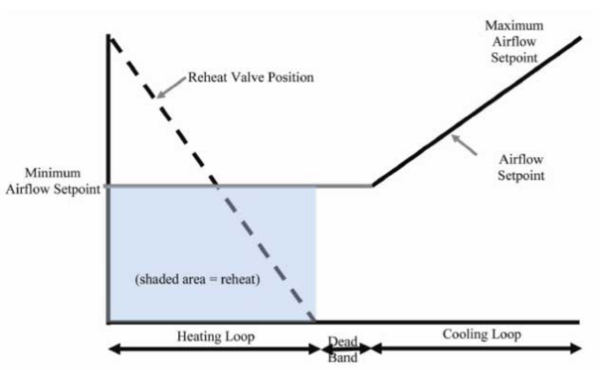
\includegraphics[width=0.9\textwidth, height=0.9\textheight, keepaspectratio=true]{media/image264.png}
\caption{The Single Maximum Control Logic \protect \label{fig:the-single-maximum-control-logic}}
\end{figure}

With \textbf{Reverse} and \textbf{ReverseWithLimits} (the default) action, as the heating load increases, the unit starts at minimum air flow and minimum hot water flow. The hot water flow is increased until it reaches maximum flow or the user-specified maximum reheat air temperature is reached, then the air damper starts to open to meet the load. For \textbf{Reverse} the damper can open all the way. For \textbf{ReverseWithLimits}s the damper can only partially open to a maximum flow rate given by the following two fields. These options are used if the minimum air flow rate is not adequate to serve the peak heating load. This is sometimes called the dual maximum control logic as illustrated in following figure. For heating coil types other than the hot-water coil, e.g.~electric, steam, and gas, the reverse action works the same as the normal action -- always keeping the air flow at the minimum during heating.

The dual-max control currently applies to the AirTerminal:SingleDuct:VAV:Reheat objects with reverse acting dampers and hot-water coils.

\begin{figure}[hbtp] % fig 103
\centering
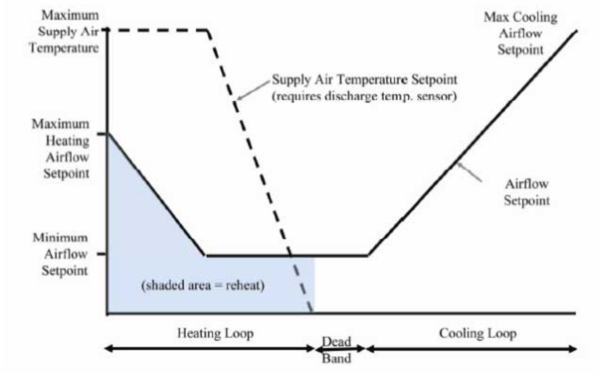
\includegraphics[width=0.9\textwidth, height=0.9\textheight, keepaspectratio=true]{media/image265.png}
\caption{  The Dual Maximum Control Logic \protect \label{fig:the-dual-maximum-control-logic}}
\end{figure}

\paragraph{Control Fields for Maximum Flow During Reheat:}\label{control-fields-for-maximum-flow-during-reheat}

The following two fields are used only when Reheat Coil Object Type = \hyperref[coilheatingwater]{Coil:Heating:Water} and Damper Heating Action = ReverseWithLimits. Maximum Flow per Zone Floor Area During Reheat and Maximum Flow Fraction During Reheat are two optional methods to calculate the maximum allowable air flow rate during reheat operation. If both are entered, the greater resulting flow rate is used. If Design Specification Outdoor Air Object Name is also specified, it may increase this limit to meet the outdoor air flow rate requirement. At no time will the maximum flow rate calculated here exceed the value for Maximum Air Flow Rate.

This limit is active only when the zone thermostat requests heating and the VAV box damper is reverse acting (i.e., ReverseWithLimits).

\paragraph{Field: Maximum Flow per Zone Floor Area During Reheat}\label{field-maximum-flow-per-zone-floor-area-during-reheat}

This factor (m\(^{3}\)/s-m\(^{2}\)) is multiplied by the zone area, to determine the maximum volume flow rate (m\(^{3}\)/s) allowed during reheat operation (see detailed explanation above). This field is autosizable and its default is autosize. If autosize is selected or the field is blank, the value is filled from the similar inputs in \hyperref[sizingzone]{Sizing:Zone}. If there is no sizing calculation the value is set to 0.002032 m\(^{3}\)/s-m\(^{2}\) (0.4 cfm/ft\(^{2}\)). If this field and the following field are entered, the greater of the two inputs is used. This field and the following field are only used if Damper Heating Action = ReverseWithLimits.

\paragraph{Field: Maximum Flow Fraction During Reheat}\label{field-maximum-flow-fraction-during-reheat}

This fraction is multiplied by the Maximum Air Flow Rate to determine the maximum volume flow rate (m\(^{3}\)/s) allowed during reheat operation (see detailed explanation above). This field is autosizeable and is defaulted to autosize. If autosizeable is selected or the field is blank, the value is set to 0.002032 m\(^{3}\)/s-m\(^{2}\) (0.4 cfm/ft\(^{2}\)) multiplied by the zone floor area divided by the Maximum Air Flow Rate. If this field and the previous field are entered, the greater of the two inputs is used. This field and the following field are only used if Damper Heating Action = ReverseWithLimits.

\paragraph{Field: Maximum Reheat Air Temperature}\label{field-maximum-reheat-air-temperature-1}

This field specifies a maximum supply air temperature (°C) leaving the reheat coil in a VAV terminal unit during heating operation. If leaving blank, the temperature of the supply air to the space in heating operation may get unrealistic high.

\paragraph{Field: Design Specification Outdoor Air Object Name}\label{field-design-specification-outdoor-air-object-name}

This alpha field specifies the name of a \hyperref[designspecificationoutdoorair]{DesignSpecification:OutdoorAir} or \hyperref[designspecificationoutdoorairspacelist]{DesignSpecification:OutdoorAir:SpaceList} object. When this field is used, the terminal unit will increase flow as needed to meet this outdoor air requirement. If Outdoor Air Flow per Person is non-zero, then the outdoor air requirement will be computed based on the current number of occupants in the zone. At no time will the supply air flow rate exceed the value for Maximum Air Flow Rate. If this field is blank, then the terminal unit will not be controlled for outdoor air flow. See documentation for the zone HVAC outdoor air object for further information (Ref \hyperref[designspecificationoutdoorair]{DesignSpecification:OutdoorAir}).

\paragraph{Field: Minimum Air Flow Turndown Schedule Name}

This field adjusts the \textit{Constant Minimum Air Flow Fraction}, \textit{Fixed Minimum Air Flow Rate}, or \textit{Minimum Air Flow Fraction Schedule} value by multiplying it using this schedule. Schedule values are fractions, 0.0 to 1.0. This field adjusts the minimum airflow turndown value below the zone design minimum air flow and is intended for use with ASHRAE Standard 170. This field can also be used to adjust the design minimum air flow sizing calculation by applying a desired fraction values to summer and winter design days turndown schedule. If this field is left blank, then the turndown minimum air flow fraction value is set to 1.

An IDF example:

\begin{lstlisting}

    AirTerminal:SingleDuct:VAV:Reheat,
      SPACE2-1 VAV Reheat,  !- Name of System
      ReheatCoilAvailSched,  !- Availability schedule for VAV System
      SPACE2-1 Zone Coil Air In Node,  !- Damper Air Outlet Node
      SPACE2-1 ATU In Node,  !- Unit Air Inlet Node
      autosize,  !- Maximum air flow rate {m3/s}
      Constant,  !- Zone Minimum Air Flow Input Method
      0.3,  !- Constant Minimum Air Flow Fraction
      ,  !- Fixed Minimum Air Flow Rate
      ,  !- Minimum Air Flow Fraction Schedule Name
      COIL:Gas:Heating,  !- Reheat Component Object
      SPACE2-1 Zone Coil,  !- Name of Reheat Component
      0.0,  !- Max Reheat Water Flow {m3/s}
      0.0,  !- Min Reheat Water Flow {m3/s}
      SPACE2-1 In Node,  !- Unit Air Outlet Node
      0.001,  !- Convergence Tolerance
      ReverseWithLimits,  !- Damper Heating Action
      ,         !- Maximum Flow per Zone Floor Area During Reheat
      ,         !- Maximum Flow Fraction During Reheat
      35.0,     !- Maximum Reheat Air Temperature {C}
      ,         !- Design Specification Outdoor Air Object Name
      TurndownMinAirFlowSch;   !- Minimum Air Flow Turndown Schedule Name

    DesignSpecification:OutdoorAir,
      ZoneMinOARequirements,    !- Name
      Sum,                      !- Outdoor Air Method
      0.00472,                  !- Outdoor Air Flow per Person {m3/s}
      0.000508,                 !- Outdoor Air Flow per Zone Floor Area {m3/s-m2}
      ,                         !- Outdoor Air Flow per Zone
      ,                         !- Outdoor Air Flow Air Changes per Hour
      Min OARequirements Sched; !- Outdoor Air Flow Rate Fraction Schedule Name

    Schedule:Compact,
      Min OARequirements Sched,  !- Name
      Any Number,                !- Schedule Type Limits Name
      Through: 12/31,            !- Field 1
      For: Weekdays SummerDesignDay WinterDesignDay, !- Field 2
      Until: 24:00,1.0,          !- Field 7
      For: AllOtherDays,         !- Field 9
      Until: 24:00,0.25;         !- Field 10

    COIL:Heating:Fuel,
      SPACE1-1 Zone Coil,  !- Coil Name
      ReheatCoilAvailSched,  !- Availability Schedule Name
      NaturalGas,             !- Fuel Type
      0.8,  !- Gas Burner Efficiency of the Coil
      autosize,  !- Nominal Capacity of the Coil {W}
      SPACE1-1 Zone Coil Air In Node,  !- Coil_Air_Inlet_Node
      SPACE1-1 In Node;  !- Coil_Air_Outlet_Node

    Schedule:Compact,
      TurndownMinAirFlowSch,   !- Name
      Fraction,                !- Schedule Type Limits Name
      Through: 12/31,          !- Field 1
      For: Weekdays,           !- Field 2
      Until: 7:00,0.50,        !- Field 3
      Until: 17:00,0.75,       !- Field 4
      Until: 24:00,0.50,       !- Field 5
      For: SummerDesignDay WinterDesignDay, !- Field 6
      Until: 24:00,1.0,        !- Field 7
      For: Weekends Holidays CustomDay1 CustomDay2, !- Field 8
      Until: 24:00,0.25;       !- Field 9
\end{lstlisting}

\subsubsection{Outputs}\label{outputs-2-000}

\begin{itemize}
\item
  HVAC,Average,Zone Air Terminal VAV Damper Position {[]}
\item
  HVAC,Average,Zone Air Terminal Minimum Air Flow Fraction {[]}
\item
  HVAC,Average,Zone Air Terminal Outdoor Air Volume Flow Rate {[}m3/s{]}
\end{itemize}

\paragraph{Zone Air Terminal VAV Damper Position {[]}}\label{zone-air-terminal-vav-damper-position}

This output is the variable air volume damper position required to meet the zone load. This is the average value over the frequency being reported. The damper position is defined as the terminal unit air mass flow rate divided by the terminal unit's maximum air mass flow rate.

\paragraph{Zone Air Terminal Minimum Air Flow Fraction {[]}}\label{zone-air-terminal-minimum-air-flow-fraction}

This output is the value for the minimum air flow fraction setting on a VAV terminal.~~ This is the average value over the frequency being reported. The minimum air flow fraction is defined as the lower limit on the terminal unit air mass flow rate divided by the terminal units maximum air mass flow rate.

\paragraph{Zone Air Terminal Outdoor Air Volume Flow Rate {[}m3/s{]}}

This output is the amount of outdoor air entering the zone. This is the average value over the frequency being reported. The amount of outdoor air is defined as the terminal unit air volume flow rate multiplied by the fraction of outdoor air entering the air loop's outside air system.

\subsection{AirTerminal:SingleDuct:VAV:Reheat:VariableSpeedFan}\label{airterminalsingleductvavreheatvariablespeedfan}

The VAV terminal unit with variable-speed fan and reheat coil is an air system terminal unit consisting of a variable speed fan in series with a heating coil. These units are usually employed in underfloor air distribution (UFAD) systems where the air is supplied at low static pressure through an underfloor plenum. The fan is used to control the flow of conditioned air that enters the space. When the fan is off the plenum pressure drives the minimum air flow through the terminal unit. At maximum cooling the fan runs at its maximum speed. At full heating the fan runs at its heating maximum -- usually less than the cooling maximum flow rate. Thus this unit has two separate maximum flow rates -- one for heating and one for cooling.

For cooling, control is maintained simply by varying the fan speed. For heating, the unit first tries to meet the heating load by varying the heating coil output while keeping the air flow at minimum (fan off). If this is not adequate the fan turns on and operates in variable flow mode up to the heating maximum flow rate. The zone fan-off minimum supply air flow can be further adjusted using scheduled fraction values specified in the field \textit{Minimum Air Flow Turndown Schedule Name}.

This unit is modeled in EnergyPlus as a compound component -- a variable speed fan and a heating coil in series in the air stream. The unit is blow through -- the fan is upstream of the heating coil.

\subsubsection{Inputs}\label{inputs-3-000}

\paragraph{Field: Name}\label{field-name-3-000}

A unique user assigned name for a particular VS fan VAV reheat terminal unit. Any reference to this unit by another object will use this name.

\paragraph{Field: Availability Schedule Name}\label{field-availability-schedule-name-3}

The name of the schedule (ref: Schedule) that denotes whether the unit can run during a given time period. A schedule value greater than 0 (usually 1 is used) indicates that the unit can be on during the time period. A value less than or equal to 0 (usually 0 is used) denotes that the unit must be off for the time period. If this field is blank, the schedule has values of 1 for all time periods.

\paragraph{Field: Maximum Cooling Air Flow Rate}\label{field-maximum-cooling-air-flow-rate}

The maximum volumetric air flow rate through the unit in cubic meters per second when the thermostat is calling for cooling. Normally this is the same as the unit's fan maximum volumetric flow rate.

\paragraph{Field: Maximum Heating Air Flow Rate}\label{field-maximum-heating-air-flow-rate}

The maximum volumetric air flow rate through the unit in cubic meters per second when the thermostat is calling for heating.

\paragraph{Field: Zone Minimum Air Flow Fraction}\label{field-zone-minimum-air-flow-fraction}

The minimum flow rate to the zone while the system is operating, specified as a fraction of the maximum air flow rate. For this unit this is the flow rate when the fan is off.

\paragraph{Field: Air Inlet Node Name}\label{field-air-inlet-node-name-2}

The name of the HVAC system node that is the air inlet node for the terminal unit. This is also the air inlet node for the unit's fan.

\paragraph{Field: Air Outlet Node Name}\label{field-air-outlet-node-name-2}

The name of the HVAC system node that is the air outlet node of the unit. This same node will be the unit heating coil's air outlet node. This node is also a zone inlet node.

\paragraph{Field: Fan Object Type}\label{field-fan-object-type}

The type of fan in the terminal unit. At this time the only type of fan allowed is \emph{\hyperref[fansystemmodel]{Fan:SystemModel}} or \emph{\hyperref[fanvariablevolume]{Fan:VariableVolume}}.

\paragraph{Field: Fan Name}\label{field-fan-name}

The name of the particular fan object in this terminal unit.

\paragraph{Field: Heating Coil Object Type}\label{field-heating-coil-object-type}

The type of heating coil in the terminal unit. The valid choices are:

\begin{itemize}
\item
  \hyperref[coilheatingwater]{Coil:Heating:Water}
\item
  \hyperref[coilheatingelectric]{Coil:Heating:Electric}
\item
  \hyperref[coilheatinggas-000]{Coil:Heating:Fuel}
\item
  \hyperref[coilheatingsteam]{Coil:Heating:Steam}
\end{itemize}

\paragraph{Field: Heating Coil Name}\label{field-heating-coil-name}

The name of the heating coil object contained in this terminal unit.

\paragraph{Field: Maximum Hot Water or Steam Flow Rate}\label{field-maximum-hot-water-or-steam-flow-rate-2}

The maximum hot water or steam volumetric flow rate in m\(^{3}\)/s through the unit's heating coil. The steam volumetric flow rate is calculated at 100C and 101325 Pa. If the heating coil is not a hot water or steam coil this field should be left blank.

\paragraph{Field: Minimum Hot Water or Steam Flow Rate}\label{field-minimum-hot-water-or-steam-flow-rate-2}

The minimum hot water or steam volumetric flow rate in m\(^{3}\)/s through the unit's heating coil. The steam volumetric flow rate is calculated at 100C and 101325 Pa. If the heating coil is not a hot water or steam coil this field should be left blank.

\paragraph{Field: Heating Convergence Tolerance}

The control tolerance for the unit heating output. The unit is controlled by matching the unit output to the zone demand. The model must be numerically inverted to obtain a specified output. The convergence tolerance is the error tolerance used to terminate the numerical inversion procedure. Basically, this is the fraction:

\begin{equation}
  \frac{\left| Q_{\rm{unit, out}} - Q_{\rm{zone load}} \right|}{Q_{\rm{zone load}}} \le \rm{ConvergenceTolerance}
\end{equation}

% \begin{equation}
%   \frac{\left| Q_{\rm{PIU, out}} - Q_{\rm{zone load}} \right|}{Q_{\rm{zone load}}} \le \rm{ConvergenceTolerance}
% \end{equation}

The default is 0.001.

\paragraph{Field: Minimum Air Flow Turndown Schedule Name}

This field adjusts \textit{Zone Minimum Air Flow Fraction} by multiplying it using this schedule. Schedule values are fractions, 0.0 to 1.0. This field adjusts the minimum airflow turndown value below the zone design minimum air flow and is intended for use with ASHRAE Standard 170. This field can also be used to adjust the design minimum air flow sizing calculation by applying a desired fraction values to summer and winter design days turndown schedule. If this field is left blank, then the turndown minimum air flow fraction value is set to 1 and the VAV air terminal uses the fixed fraction specified in in the field \textit{Zone Minimum Air Flow Fraction}.

An IDF example:

\begin{lstlisting}
AirTerminal:SingleDuct:VAV:Reheat:VariableSpeedFan,
  SPACE2-1 VAV Reheat,                  !- Name of System
  ReheatCoilAvailSched,                 !- System Availability schedule
  autosize,                             !- Maximum cooling air volume flow rate
  autosize,                             !- Maximum heating air volume flow rate
  0.05,                                 !- Zone Minimum Air Flow Fraction
  SPACE2-1 ATU In Node,                 !- Air Inlet Node Name
  SPACE2-1 In Node,                     !- Air Outlet Node Name
  FAN:VariableVolume,                   !- Fan object
  SPACE2-1 Zone Fan,                    !- Fan name
  COIL:Water:SimpleHeating,             Heating coil object
  SPACE2-1 Zone Coil,                   !- Heating coil name
  autosize,                             !- Max hot water flow
  0.0,                                  !- Min hot water flow
  0.001,                                !- Heating Convergence Tolerance
  TurndownMinAirFlowSch;   !- Minimum Air Flow Turndown Schedule Name

Coil:Heating:Water,
  SPACE2-1 Zone Coil,                   !- Coil Name
  ReheatCoilAvailSched,                 !- Availability Schedule Name
  autosize,                             !- UA of the Coil {W/K}
  autosize,                             !- Max Water Flow Rate of Coil {m3/s}
  SPACE2-1 Zone Coil Water In Node,     !- Coil_Water_Inlet_Node
  SPACE2-1 Zone Coil Water Out Node,    !- Coil_Water_Outlet_Node
  SPACE2-1 Zone Coil Air In Node,       !- Coil_Air_Inlet_Node
  SPACE2-1 In Node;                     !- Coil_Air_Outlet_Node

Fan:VariableVolume,
  SPACE2-1 Zone Fan,                    !- Fan Name
  FanAvailSched,                        !- Availability Schedule Name
  0.7,                                  !- Fan Total Efficiency
  125.0,                                !- Delta Pressure {Pa}
  autosize,                             !- Max Flow Rate {m3/s}
  0.0,                                  !- Min Flow Rate {m3/s}
  0.9,                                  !- Motor Efficiency
  1.0,                                  !- Motor In Airstream Fraction
  0.00153028,                           !- FanCoefficient 1
  0.00520806,                           !- FanCoefficient 2
  1.1086242,                            !- FanCoefficient 3
  -.11635563,                           !- FanCoefficient 4
  0.000,                                !- FanCoefficient 5
  SPACE2-1 ATU In Node,                 !- Fan_Inlet_Node
  SPACE2-1 Zone Coil AirIn Node;        !- Fan_Outlet_Node

Schedule:Compact,
  TurndownMinAirFlowSch,   !- Name
  Fraction,                !- Schedule Type Limits Name
  Through: 12/31,          !- Field 1
  For: Weekdays,           !- Field 2
  Until: 7:00,0.50,        !- Field 3
  Until: 17:00,0.75,       !- Field 4
  Until: 24:00,0.50,       !- Field 5
  For: SummerDesignDay WinterDesignDay, !- Field 6
  Until: 24:00,1.0,        !- Field 7
  For: Weekends Holidays CustomDay1 CustomDay2, !- Field 8
  Until: 24:00,0.25;       !- Field 9
\end{lstlisting}

\subsubsection{Outputs}\label{outputs-3}

\begin{itemize}
\item
  HVAC,Average,Zone Air Terminal VAV Damper Position {[]}
\item
  HVAC,Average,Zone Air Terminal Outdoor Air Volume Flow Rate {[}m3/s{]}
\end{itemize}

\paragraph{Zone Air Terminal VAV Damper Position}\label{zone-air-terminal-vav-damper-position-1}

This output is the variable air volume flow fraction required to meet the zone load. This is the average value over the frequency being reported. The flow fraction is defined as the terminal unit air mass flow rate divided by the terminal unit's maximum air mass flow rate.

\paragraph{Zone Air Terminal Outdoor Air Volume Flow Rate {[}m3/s{]}}

This output is the amount of outdoor air entering the zone. This is the average value over the frequency being reported. The amount of outdoor air is defined as the terminal unit air volume flow rate multiplied by the fraction of outdoor air entering the air loop's outside air system.

\subsection{AirTerminal:SingleDuct:VAV:HeatAndCool:Reheat}\label{airterminalsingleductvavheatandcoolreheat}

Variable air volume (VAV) systems typically control the dry-bulb temperature inside a zone by varying the supply air volume instead of the supply air temperature (ref: \hyperref[airterminalsingleductvavnoreheat]{AirTerminal:SingleDuct:VAV:NoReheat}). Reheat coils may be required to avoid overcooling (ref: \hyperref[airterminalsingleductvavreheat]{AirTerminal:SingleDuct:VAV:Reheat}).

This terminal unit is slightly different from the \hyperref[airterminalsingleductvavreheat]{AirTerminal:SingleDuct:VAV:Reheat} terminal unit. Both operate the same in cooling mode: the damper opens as needed to provide additional sensible cooling to the zone. The difference between the two is in heating mode.~ For the Single Duct VAV Reheat terminal unit, the air flow rate is reduced to the minimum value (max air flow rate x zone minimum air flow fraction) when zone heating is required and the reheat coil output is modulated to meet the zone heating load. The zone minimum supply air flow can be further adjusted using scheduled fraction values specified in the field \textit{Minimum Air Flow Turndown Schedule Name}.~ For the AirTerminal:SingleDuct:VAV:HeatAndCool:Reheat terminal unit, the air flow rate in heating mode is increased to meet higher zone heating loads (similar to what is done in cooling mode). If additional heat is required (beyond what the terminal unit can provide with its damper fully open), then the reheat coil is modulated as needed to meet the additional heating load.

This terminal unit model was originally developed and tested for use with the changeover-bypass VAV unitary system.

\begin{figure}[hbtp] % fig 104
\centering
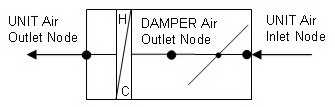
\includegraphics[width=0.9\textwidth, height=0.9\textheight, keepaspectratio=true]{media/image267.png}
\caption{Single Duct VAV Heat and Cool Reheat Schematic \protect \label{fig:single-duct-vav-heat-and-cool-reheat}}
\end{figure}

\subsubsection{Inputs}\label{inputs-4-000}

\paragraph{Field: Name}\label{field-name-4-000}

Unique user-defined name for this Air Distribution Unit (ADU).

\paragraph{Field: Availability Schedule Name}\label{field-availability-schedule-name-4}

This alpha field defines the name of the schedule (ref: Schedule) that denotes whether or not this component is available to operate during a given time period. A schedule value greater than 0 (usually 1 is used) indicates that the component can be on during the time period. A value less than or equal to 0 (usually 0 is used) denotes that the component must be off for the time period. If this field is blank, the schedule has values of 1 for all time periods.

\paragraph{Field: Damper Air Outlet Node Name}\label{field-damper-air-outlet-node-name-1}

This alpha field defines the name of the VAV damper air outlet node. This is the outlet node of the damper and the inlet node of the reheat coil.

\paragraph{Field: Air Inlet Node Name}\label{field-air-inlet-node-name-3}

This alpha field defines the name of the air inlet node that connects the air splitter to the individual zone ADU. This is \emph{not} the same as the air inlet node of the reheat component: it is upstream of that node. This is the inlet node to the terminal unit and the damper.

\paragraph{Field: Maximum Air Flow Rate}\label{field-maximum-air-flow-rate-3}

This numeric field defines the design maximum volumetric flow rate (m\(^{3}\)/sec) specified for this VAV ADU. This flow rate must be greater than 0 or can be autosized.

\paragraph{Field: Zone Minimum Air Flow Fraction}\label{field-zone-minimum-air-flow-fraction-1}

This numeric field defines the minimum air volumetric flow rate to the zone while the system is operating, specified as a fraction of the maximum air flow rate. The minimum zone fraction is normally specified to meet the minimum ventilation requirement for the occupants. The reheat coil operates as needed to maintain the heating set point specified in the Zone Control:Thermostatic object. This value must be between 0 and 1.

\paragraph{Field: Reheat Coil Object Type}\label{field-reheat-coil-object-type-2}

The valid reheat component objects currently available are:

\begin{itemize}
\item
  \hyperref[coilheatingwater]{Coil:Heating:Water}
\item
  \hyperref[coilheatingelectric]{Coil:Heating:Electric}
\item
  \hyperref[coilheatinggas-000]{Coil:Heating:Fuel}
\item
  \hyperref[coilheatingsteam]{Coil:Heating:Steam}
\end{itemize}

If no reheat coil is required, use \hyperref[airterminalsingleductvavheatandcoolnoreheat]{AirTerminal:SingleDuct:VAV:HeatAndCool:NoReheat} instead of this object.

\paragraph{Field: Reheat Coil Name}\label{field-reheat-coil-name-2}

Unique coil name being simulated with this ADU. Applicable for all coils. If there is no reheat coil, use \hyperref[airterminalsingleductvavheatandcoolnoreheat]{AirTerminal:SingleDuct:VAV:HeatAndCool:NoReheat} instead of this object.

\paragraph{Field: Maximum Hot Water or Steam Flow Rate}\label{field-maximum-hot-water-or-steam-flow-rate-3}

This field is ignored for gas or electric reheat coils. If using a hot water or steam reheat coil, set to the maximum design water or steam volumetric flow rate in m\(^{3}\)/s for the hot water or steam heating coil. The steam volume flow rate is calculated at 100C and 101325 Pa. This volumetric flow rate can be autosized.

\paragraph{Field: Minimum Hot Water or Steam Flow Rate}\label{field-minimum-hot-water-or-steam-flow-rate-3}

This field is ignored for gas and electric coils. Set to the minimum design water or steam volumetric flow rate in m\(^{3}\)/s for the hot water or steam heating coil, normally set to be a shut-off valve that is set to zero. The steam volume flow rate is calculated at 100C and 101325 Pa.

\paragraph{Field: Air Outlet Node Name}\label{field-air-outlet-node-name-3}

This is the air outlet node for the ADU and is then connected to the zone. This is the same node as the air outlet node of the reheat component.

\paragraph{Field: Convergence Tolerance}\label{field-convergence-tolerance-2}

The coil is controlled by knowing the zone demand determined by the zone thermostat and setting the outlet conditions to meet this demand. For the electric and gas coils, this is set exactly since the coil model solution can be inverted and this field is not used. With the hot water coil that uses an effectiveness-NTU method, the solution cannot be inverted directly. Therefore, to determine the correct mass flow rate for the hot water the solution is solved by iteration. The iterative solution uses an interval-halving routine and needs a termination criterion that is set with this Convergence Tolerance parameter. This control offset is set to a decimal fraction of the zone demand. The default value for this field is 0.001.

\paragraph{Field: Maximum Reheat Air Temperature}\label{field-maximum-reheat-air-temperature-2}

This is the upper limit on the temperature in degrees C of the air leaving the terminal unit -- reheat coil (and being delivered to the zone). If the user leaves this field blank, no maximum reheat air temperature is enforced.

\paragraph{Field: Minimum Air Flow Turndown Schedule Name}

This field adjusts the \textit{Zone Minimum Air Flow Fraction} by multiplying it using this schedule. Schedule values are fractions, 0.0 to 1.0. This field adjusts the minimum airflow turndown value below the zone design minimum air flow and is intended for use with ASHRAE Standard 170. This field can also be used to adjust the design minimum air flow sizing calculation by applying a desired fraction values to summer and winter design days turndown schedule. If this field is left blank, then the turndown minimum air flow fraction value is set to 1 and uses the fixed fraction specified in the field \textit{Zone Minimum Air Flow Fraction}.

An IDF example is provided below:

\begin{lstlisting}

AirTerminal:SingleDuct:VAV:HeatAndCool:Reheat,
      Zone 1 VAV System,             !- Name of System
      FanAndCoilAvailSched,          !- System Availability schedule
      Zone 1 Reheat Air Inlet Node,  !- DAMPER Air Outlet Node
      Zone 1 VAV Inlet Node,         !- UNIT Air Inlet Node
      0.583,                         !- Maximum air flow rate {m3/s}
      0.25,                          !- Zone Minimum Air Flow Fraction
      Coil:Heating:Electric,         !- Reheat Component Object
      Reheat Coil Zone 1,            !- Name of Reheat Component
      0.0,                           !- Max Reheat Water Flow {m3/s}
      0.0,                           !- Min Reheat Water Flow {m3/s}
      Zone 1 Reheat Air Outlet Node, !- UNIT Air Outlet Node
      0.001;                         !- Convergence Tolerance

  Coil:Heating:Electric,
      Reheat Coil Zone 1,            !- Coil Name
      FanAndCoilAvailSched,          !- Availability Schedule Name
      1.0,                           !- Efficiency of the Coil
      3000.0,                        !- Nominal Capacity of the Coil {W}
      Zone 1 Reheat Air Inlet Node,  !- Coil_Air_Inlet_Node
      Zone 1 Reheat Air Outlet Node; !- Coil_Air_Outlet_Node
\end{lstlisting}

\subsubsection{Outputs}\label{outputs-4}

\begin{itemize}
\item
  HVAC,Average,Zone Air Terminal VAV Damper Position {[]}
\item
  HVAC,Average,Zone Air Terminal Outdoor Air Volume Flow Rate {[}m3/s{]}
\end{itemize}

\paragraph{Zone Air Terminal VAV Damper Position {[]}}\label{zone-air-terminal-vav-damper-position-2}

This output is the damper position required to meet the zone load. This is the average value over the simulation timestep being reported. The damper position is defined as the terminal unit air mass flow rate divided by the terminal unit's maximum air mass flow rate.

\paragraph{Zone Air Terminal Outdoor Air Volume Flow Rate {[}m3/s{]}}

This output is the amount of outdoor air entering the zone. This is the average value over the frequency being reported. The amount of outdoor air is defined as the terminal unit air volume flow rate multiplied by the fraction of outdoor air entering the air loop's outside air system.

\subsection{AirTerminal:SingleDuct:VAV:NoReheat}\label{airterminalsingleductvavnoreheat}

Variable air volume (VAV) systems control the dry-bulb temperature inside a zone by varying the supply air volume instead of the air temperature. At full cooling the VAV damper is fully open supplying the specified maximum air flow rate. As the cooling load decreases, the damper closes until it reaches the minimum stop specified by the zone minimum air flow fraction. The zone minimum supply air flow can be adjusted using scheduled fraction values specified in the field \textit{Minimum Air Flow Turndown Schedule Name}.

VAV systems can be used for interior or perimeter zones with a common fan system and air temperature control. The VAV concept may vary according to the VAV box locations and air temperature controls. Heating can be provided if necessary by use of baseboard.

\subsubsection{Inputs}\label{inputs-5-000}

\paragraph{Field: Name}\label{field-name-5-000}

Unique name for the VAV Air Distribution Unit (ADU).

\paragraph{Field: Availability Schedule Name}\label{field-availability-schedule-name-5}

Schedule that this component will operate or is available to operate. A schedule value greater than 0 (usually 1 is used) indicates that the component can be on during the time period. A value less than or equal to 0 (usually 0 is used) denotes that the component must be off for the time period. If this field is blank, the schedule has values of 1 for all time periods.

\paragraph{Field: Air Outlet Node Name}\label{field-air-outlet-node-name-4}

The VAV damper and Unit outlet node.

\paragraph{Field: Air Inlet Node Name}\label{field-air-inlet-node-name-4}

The air inlet node name that connects the air splitter to the individual zone ADU.

\paragraph{Field: Maximum Air Flow Rate}\label{field-maximum-air-flow-rate-4}

The design maximum volume flow rate (m\(^{3}\)/sec) specified for VAV ADU. This is autosizable.

\paragraph{Field: Zone Minimum Air Flow Method}\label{field-zone-minimum-air-flow-method-1}

This field is used to select how the program will determine the minimum flow rate to the zone while the system is operating.~ The minimum flow rate is modeled as a fraction of the maximum flow rate.~ There are three choices for selecting how the minimum flow rate is specified:~ Constant, FixedFlowRate, and Scheduled.~ If Constant is entered, then the program will use the value for the constant minimum air flow fraction entered in the following field.~ If FixedFlowRate is entered, then the program will use the value for minimum flow rate entered in the field below called Fixed Minimum Air Flow Rate.~ If Scheduled is entered, then the program will obtain the value for minimum flow fraction from the schedule named in the field below called Minimum Air Flow Fraction Schedule Name. The default is Constant.

\paragraph{Field: Constant Minimum Air Flow Fraction}\label{field-constant-minimum-air-flow-fraction-1}

The minimum flow rate to the zone while the system is operating, specified as a fraction of the maximum air flow rate. The minimum zone fraction is normally specified to meet the minimum ventilation requirement for the occupants. This field is only used if the Zone Minimum Air Flow Method field is set to Constant.

This field is autosizable and defaulted to autosize. If a Sizing:System \emph{System Outdoor Air Method} other than Standard62.1SimplifiedProcedure is specified, the autosized flow fraction is calculated using the maximum flow rate derived from the design outdoor air flow (including VRP adjustments) and the \hyperref[sizingzone]{Sizing:Zone} input fields ``Cooling Minimum Air Flow per Zone Floor Area'', ``Cooling Minimum Air Flow'', and ``Cooling Minimum Air Flow Fraction''. If there is no sizing calculation the defaults of 0.000762 cubic meters per second per square meter of zone floor area (0.15 cfm/ft2) and 0.2 are used. The autosized flow fraction is calculated according to the ASHRAE Standard 62.1 Simplified Procedure if the Sizing:System's ``System Outdoor Air Method'' associated with this terminal is set to Standard62.1SimplifiedProcedure.

\paragraph{Field: Fixed Minimum Air Flow Rate}\label{field-fixed-minimum-air-flow-rate-1}

The minimum flow rate to the zone while the system is operating, specified as a fixed minimum air flow rate in meters cubed per second. The minimum air flow rate is normally specified to meet the minimum ventilation requirement for the occupants. This field is only used if the Zone Minimum Air Flow Method field is set to FixedFlowRate.

This field is autosizable and defaulted to autosize. The autosized flow rate is the maximum flow rate derived from the design outdoor air flow (including VRP adjustments) and the \hyperref[sizingzone]{Sizing:Zone} input fields ``Cooling Minimum Air Flow per Zone Floor Area'', ``Cooling Minimum Air Flow'', and ``Cooling Minimum Air Flow Fraction''. If there is no sizing calculation the defaults of 0.000762 cubic meters per second per square meter of zone floor area (0.15 cfm/ft2) and 0.2 flow fraction are used. The autosized flow rate is calculated according to the ASHRAE Standard 62.1 Simplified Procedure if the Sizing:System's ``System Outdoor Air Method'' associated with this terminal is set to Standard62.1SimplifiedProcedure.

\paragraph{Field: Minimum Air Flow Fraction Schedule Name}\label{field-minimum-air-flow-fraction-schedule-name-1}

The name of a schedule that determines the value of the minimum air flow fraction.~ The schedule should contain fractions from 0.0 to 1.0.~ These values will define the minimum flow rate to the zone while the system is operating, specified as a fraction of the maximum air flow rate. This field is only used if the Zone Minimum Air Flow Method field is set to Scheduled.

\paragraph{Field: Design Specification Outdoor Air Object Name}\label{field-design-specification-outdoor-air-object-name-1}

This alpha field specifies the name of a \hyperref[designspecificationoutdoorair]{DesignSpecification:OutdoorAir} or \hyperref[designspecificationoutdoorairspacelist]{DesignSpecification:OutdoorAir:SpaceList} object. When this field is used, the terminal unit will increase flow as needed to meet this outdoor air requirement. If Outdoor Air Flow per Person is non-zero, then the outdoor air requirement will be computed based on the current number of occupants in the zone. At no time will the supply air flow rate exceed the value for Maximum Air Flow Rate. If this field is blank, then the terminal unit will not be controlled for outdoor air flow. See documentation for the zone HVAC outdoor air object for further information (Ref \hyperref[designspecificationoutdoorair]{DesignSpecification:OutdoorAir}).

\paragraph{Field: Minimum Air Flow Turndown Schedule Name}

This field adjusts the \textit{Constant Minimum Air Flow Fraction}, \textit{Fixed Minimum Air Flow Rate}, or \textit{Minimum Air Flow Fraction Schedule} value by multiplying it using this schedule. Schedule values are fractions, 0.0 to 1.0. This field adjusts the minimum airflow turndown value below the zone design minimum air flow and is intended for use with ASHRAE Standard 170. This field can also be used to adjust the design minimum air flow sizing calculation by applying a desired fraction values to summer and winter design days turndown schedule. If this field is left blank, then the turndown minimum air flow fraction value is set to 1.

An IDF example:

\begin{lstlisting}

  AirTerminal:SingleDuct:VAV:NoReheat,
      Zone 1 VAV System,       !- Name
      FanAndCoilAvailSched,    !- Availability Schedule Name
      Zone 1 Reheat Air Outlet Node,  !- Air Outlet Node Name
      Zone 1 Damper Inlet Node,!- Air Inlet Node Name
      0.47,                    !- Maximum Air Flow Rate {m3/s}
      Constant,                !- Zone Minimum Air Flow Input Method
      0.3,                     !- Constant Minimum Air Flow Fraction
      ,                        !- Fixed Minimum Air Flow Rate
      ,                        !- Minimum Air Flow Fraction Schedule Name
      ZoneOAData,              !- Design Specification Outdoor Air Object Name
      TurndownMinAirFlowSch;   !- Minimum Air Flow Turndown Schedule Name

    DesignSpecification:OutdoorAir,
      ZoneOAData,            !- Name
      Sum,                   !- Outdoor Air Method
      0.00236,               !- Outdoor Air Flow per Person {m3/s}
      0.00305,               !- Outdoor Air Flow per Zone Floor Area {m3/s-m2}
      ,                      !- Outdoor Air Flow per Zone {m3/s}
      ,                      !- Outdoor Air Flow Air Changes per Hour
      OARequirements Sched;  !- Outdoor Air Flow Rate Fraction Schedule Name

  Schedule:Compact,
      OARequirements Sched,    !- Name
      Any Number,              !- Schedule Type Limits Name
      Through: 12/31,          !- Field 1
      For: Weekdays SummerDesignDay WinterDesignDay,  !- Field 2
      Until: 24:00, 1.0,       !- Field 4
      For: AllOtherDays,       !- Field 5
      Until: 24:00, 0.5;       !- Field 7

    Schedule:Compact,
      TurndownMinAirFlowSch,   !- Name
      Fraction,                !- Schedule Type Limits Name
      Through: 12/31,          !- Field 1
      For: Weekdays,           !- Field 2
      Until: 7:00,0.50,        !- Field 3
      Until: 17:00,0.75,       !- Field 4
      Until: 24:00,0.50,       !- Field 5
      For: SummerDesignDay WinterDesignDay, !- Field 6
      Until: 24:00,1.0,        !- Field 7
      For: Weekends Holidays CustomDay1 CustomDay2, !- Field 8
      Until: 24:00,0.25;       !- Field 9
\end{lstlisting}

\subsubsection{Outputs}\label{outputs-5}

\begin{itemize}
\item
  HVAC,Average,Zone Air Terminal VAV Damper Position {[]}
\item
  HVAC,Average,Zone Air Terminal Outdoor Air Volume Flow Rate {[}m3/s{]}
\end{itemize}

\paragraph{Zone Air Terminal VAV Damper Position {[]}}\label{zone-air-terminal-vav-damper-position-3}

This output is the damper position required to meet the zone load. This is the average value over the simulation timestep being reported. The damper position is defined as the terminal unit air mass flow rate divided by the terminal unit's maximum air mass flow rate.

\paragraph{Zone Air Terminal Outdoor Air Volume Flow Rate {[}m3/s{]}}

This output is the amount of outdoor air entering the zone. This is the average value over the frequency being reported. The amount of outdoor air is defined as the terminal unit air volume flow rate multiplied by the fraction of outdoor air entering the air loop's outside air system.

\subsection{AirTerminal:SingleDuct:VAV:HeatAndCool:NoReheat}\label{airterminalsingleductvavheatandcoolnoreheat}

Variable air volume (VAV) systems typically control the dry-bulb temperature inside a zone by varying the supply air volume instead of the supply air temperature (ref: \hyperref[airterminalsingleductvavnoreheat]{AirTerminal:SingleDuct:VAV:NoReheat}). Reheat coils may be required to avoid overcooling (ref: \hyperref[airterminalsingleductvavreheat]{AirTerminal:SingleDuct:VAV:Reheat}).

This terminal unit is slightly different from the \hyperref[airterminalsingleductvavnoreheat]{AirTerminal:SingleDuct:VAV:NoReheat} terminal unit. Both operate the same in cooling mode: the damper opens as needed to provide additional sensible cooling to the zone. The difference between the two is in heating mode. For the Single Duct VAV NoReheat terminal unit, the air flow rate is reduced to the minimum value (max air flow rate x zone minimum air flow fraction) when zone heating is required. The zone minimum supply air flow can be further adjusted using scheduled fraction values specified in the field \textit{Minimum Air Flow Turndown Schedule Name}. For the AirTerminal:SingleDuct:VAV:HeatAndCool:NoReheat terminal unit, the air flow rate in heating mode is increased to meet higher zone heating loads (similar to what is done in cooling mode).

This terminal unit model was originally developed and tested for use with the changeover-bypass VAV unitary system. This object may be used when the central heating coil is sufficient to maintain the heating set point temperature. Additional heating may be provided, if necessary, by use of \hyperref[airterminalsingleductvavheatandcoolreheat]{AirTerminal:SingleDuct:VAV:HeatAndCool:Reheat} or ZoneHVAC:Baseboard:* objects.

\begin{figure}[hbtp] % fig 105
\centering
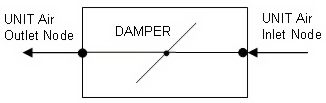
\includegraphics[width=0.9\textwidth, height=0.9\textheight, keepaspectratio=true]{media/image268.png}
\caption{Single Duct VAV Heat and Cool NoReheat Schematic \protect \label{fig:single-duct-vav-heat-and-cool-noreheat}}
\end{figure}

\subsubsection{Inputs}\label{inputs-6-000}

\paragraph{Field: Name}\label{field-name-6-000}

Unique user-defined name for this Air Distribution Unit (ADU).

\paragraph{Field: Availability Schedule Name}\label{field-availability-schedule-name-6}

This alpha field defines the name of the schedule (ref: Schedule) that denotes whether or not this component is available to operate during a given time period. If a schedule value is greater than zero then the system is available to operate; otherwise, the system is unavailable for that time period. If this field is blank, the schedule has values of 1 for all time periods.

\paragraph{Field: Air Outlet Node Name}\label{field-air-outlet-node-name-5}

This alpha field defines the name of the VAV damper air outlet node.

\paragraph{Field: Air Inlet Node Name}\label{field-air-inlet-node-name-5}

This alpha field defines the name of the air inlet node that connects the air splitter to the individual zone ADU.

\paragraph{Field: Maximum Air Flow Rate}\label{field-maximum-air-flow-rate-5}

This numeric field defines the design maximum volume flow rate (m\(^{3}\)/sec) specified for this VAV ADU. This flow rate must be greater than 0 or can be autosized.

\paragraph{Field: Zone Minimum Air Flow Fraction}\label{field-zone-minimum-air-flow-fraction-2}

This numeric field defines the minimum air volume flow rate to the zone while the system is operating, specified as a fraction of the maximum air flow rate. The minimum zone fraction is normally specified to meet the minimum ventilation requirement for the occupants. This value must be between 0 and 1.

\paragraph{Field: Minimum Air Flow Turndown Schedule Name}

This field adjusts the \textit{Zone Minimum Air Flow Fraction} by multiplying it using this schedule. Schedule values are fractions, 0.0 to 1.0. This field adjusts the minimum airflow turndown value below the zone design minimum air flow and is intended for use with ASHRAE Standard 170. This field can also be used to adjust the design minimum air flow sizing calculation by applying a desired fraction values to summer and winter design days turndown schedule. If this field is left blank, then the turndown minimum air flow fraction value is set to 1 and uses the fixed fraction specified in the field \textit{Zone Minimum Air Flow Fraction}.

An IDF example is provided below:

\begin{lstlisting}

AirTerminal:SingleDuct:VAV:HeatAndCool:NoReheat,
      Zone 3 VAV System,       !- Name of System
      FanAndCoilAvailSched,    !- System Availability schedule
      Zone 3 Reheat Air Outlet Node,  !- UNIT Air Outlet Node
      Zone 3 VAV Inlet Node,   !- UNIT Air Inlet Node
      0.584,                   !- Maximum air flow rate {m3/s}
      0.25;                    !- Zone Minimum Air Flow Fraction
\end{lstlisting}

\subsubsection{Outputs}\label{outputs-6}

\begin{itemize}
\item
  HVAC,Average,Zone Air Terminal VAV Damper Position {[]}
\item
  HVAC,Average,Zone Air Terminal Outdoor Air Volume Flow Rate {[}m3/s{]}
\end{itemize}

\paragraph{Zone Air Terminal VAV Damper Position {[]}}\label{zone-air-terminal-vav-damper-position-4}

This output is the damper position required to meet the zone load. This is the average value over the simulation timestep being reported. The damper position is defined as the terminal unit air mass flow rate divided by the terminal unit's maximum air mass flow rate.

\paragraph{Zone Air Terminal Outdoor Air Volume Flow Rate {[}m3/s{]}}

This output is the amount of outdoor air entering the zone. This is the average value over the frequency being reported. The amount of outdoor air is defined as the terminal unit air volume flow rate multiplied by the fraction of outdoor air entering the air loop's outside air system.

\subsection{AirTerminal:SingleDuct:SeriesPIU:Reheat}\label{airterminalsingleductseriespiureheat}

The series powered induction unit is an air system terminal unit that mixes varying amounts of secondary (recirculated) air and primary (conditioned supply) air to produce a fixed flow of air to a zone. The unit contains a small fan that acts to induce the secondary air and a heating coil for heating the mixed secondary and primary air. The fan runs at a constant volume flow rate whenever the unit is on (and the fan's availability schedule is on or it is activated by an availability manager). The fan is downstream of the primary and secondary air inlets. The variable mixing is accomplished by a damper in the unit's primary air supply inlet duct. This damper can move from fully open (100\% primary air. 0\% secondary air) to a minimum stop that is specified in the input description. At full cooling the damper will be fully open. At minimum cooling and for heating the damper will be at the minimum stop and the secondary air flow will be at its maximum. During night cycle operation, if the availability manager status is CycleOnZoneFansOnly, then the fan will run only if there is a heating load.  If the status is CycleOn, then the fan will run according to the normal controls.


The EnergyPlus model of the series PIU terminal unit is composed of three components: a zone mixer, a constant volume fan, and a heating coil (hot water, electric, or gas).

\begin{figure}[hbtp] % fig 106
\centering
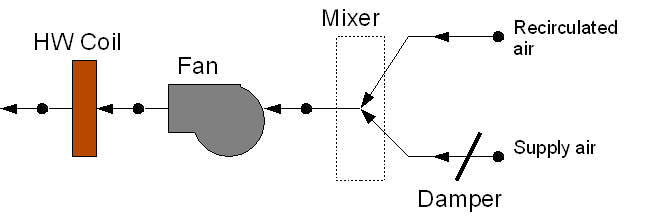
\includegraphics[width=0.9\textwidth, height=0.9\textheight, keepaspectratio=true]{media/image269.png}
\caption{Series PIU Terminal Unit \protect \label{fig:series-piu-terminal-unit}}
\end{figure}

\subsubsection{Inputs}\label{inputs-7-000}

\paragraph{Field: Name}\label{field-name-7-000}

A unique user assigned name for a particular series powered induction terminal unit. Any reference to this unit by another object will use this name.

\paragraph{Field: Availability Schedule Name}\label{field-availability-schedule-name-7}

The name of the schedule (ref: Schedule) that denotes whether the unit can run during a given time period. A schedule value greater than 0 (usually 1 is used) indicates that the unit can be on during the time period. A value less than or equal to 0 (usually 0 is used) denotes that the unit must be off for the time period. If this field is blank, the schedule has values of 1 for all time periods.

\paragraph{Field: Maximum Air Flow Rate}\label{field-maximum-air-flow-rate-6}

The maximum volumetric air flow rate through the unit in cubic meters per second. Since this is a constant air volume unit, this is also the design, rated air flow rate of the unit.

\paragraph{Field: Maximum Primary Air Flow Rate}\label{field-maximum-primary-air-flow-rate}

The maximum volumetric air flow rate of primary air through the unit in cubic meters per second. This is the primary air flow rate at full cooling load when the primary air damper is fully open. Usually this quantity is the same as the total unit flow rate, but it can be less.

\paragraph{Field: Minimum Primary Air Flow Fraction}\label{field-minimum-primary-air-flow-fraction}

The minimum volumetric air flow rate of primary air through the unit expressed as a fraction of the maximum volumetric air flow rate of primary air. This input can be 0.0. When set to autosize and the Sizing:System's \emph{System Outdoor Air Method} associated with this terminal is set to Standard62.1SimplifiedProcedure, the autosized air flow fraction is calculated according to the ASHRAE Standard 62.1 Simplified Procedure.

\paragraph{Field: Supply Air Inlet Node Name}\label{field-supply-air-inlet-node-name}

The name of the HVAC system node from which the unit draws its primary or supply air

\paragraph{Field: Secondary Air Inlet Node Name}\label{field-secondary-air-inlet-node-name}

The name of the HVAC system node from which the unit draws its secondary or recirculated air. The unit can draw secondary air from its conditioned zone directly or from a return air plenum. Thus this node should be one of the zones exhaust air nodes (see \emph{Zone Air Exhaust Node} in \textbf{\hyperref[zonehvacequipmentconnections]{ZoneHVAC:EquipmentConnections}}) or an induced air node outlet of a return plenum (see \emph{Induced Air Outlet Node} in \textbf{\hyperref[airloophvacreturnplenum]{AirLoopHVAC:ReturnPlenum}}).

\paragraph{Field: Outlet Node Name}\label{field-outlet-node-name}

The name of the HVAC system node to which the unit sends its outlet air. This should be one of the inlet air nodes of the zone which is being served.

\paragraph{Field: Reheat Coil Air Inlet Node Name}\label{field-reheat-coil-air-inlet-node-name}

The name of the HVAC system node which is the inlet node of the unit's heating coil. This is also the outlet node of the unit's fan.

\paragraph{Field: Zone Mixer Name}\label{field-zone-mixer-name}

The name of a zone mixer component (object: \hyperref[airloophvaczonemixer]{AirLoopHVAC:ZoneMixer}) which composes part of the unit. Note that some of the input for the mixer will duplicate input fields of the powered induction unit. One of the zone mixer inlet nodes should be the same as the supply air inlet node of the PIU; the other inlet node of the zone mixer should be the same as the secondary air inlet node of the PIU. The outlet node of the zone mixer should be the same as the inlet node of the PIU fan.

\paragraph{Field: Fan Name}\label{field-fan-name-1}

The name of a fan component which composes part of the unit. Note that the fan's maximum flow rate should be the same as the maximum air flow rate of the PIU and the type of fan object must be \hyperref[fansystemmodel]{Fan:SystemModel} or \hyperref[fanconstantvolume]{Fan:ConstantVolume}. The fan's inlet node should be the same as the zone mixer's outlet node. The fan's outlet node should be the same as the heating coil's air inlet node. The secondary fan will run only when the Availability Schedule specified in the fan object is >0 or when it is overridden by an availability manager (ref. \hyperref[availabilitymanagernightcycle]{AvailabilityManager:NightCycle} and others).

\paragraph{Field: Reheat Coil Object Type}\label{field-reheat-coil-object-type-3}

The type of coil in the PIU. The valid choices are:

\begin{itemize}
\item
  \hyperref[coilheatingwater]{Coil:Heating:Water}
\item
  \hyperref[coilheatingelectric]{Coil:Heating:Electric}
\item
  \hyperref[coilheatinggas-000]{Coil:Heating:Fuel}
\item
  \hyperref[coilheatingsteam]{Coil:Heating:Steam}
\end{itemize}

In other words, the PIU may have a hot water, gas, electric or steam reheat coil.

\paragraph{Field: Reheat Coil Name}\label{field-reheat-coil-name-3}

The name of the heating coil component which composes part of the unit. Note that the heating coil's air inlet node is the same as the fan outlet node and the heating coil's air outlet node is the same as the PIU outlet node.

\paragraph{Field: Maximum Hot Water or Steam Flow Rate}\label{field-maximum-hot-water-or-steam-flow-rate-4}

The maximum hot water volumetric flow rate in m\(^{3}\)/sec through the unit's heating coil. If the heating coil is gas or electric this field should be blank.

\paragraph{Field: Minimum Hot Water or Steam Flow Rate}\label{field-minimum-hot-water-or-steam-flow-rate-4}

The minimum hot water volumetric flow rate in m\(^{3}\)/sec through the unit's heating coil. If the heating coil is gas or electric this field should be blank.

\paragraph{Field: Convergence Tolerance}\label{field-convergence-tolerance-3}

The control tolerance for the unit heating output. The unit is controlled by matching the unit output to the zone demand. For units with water coils, the model must be numerically inverted to obtain a specified output. The convergence tolerance is the error tolerance used to terminate the numerical inversion procedure. Basically, this is the fraction:

\begin{equation}
\frac{{\left| {{Q_{PIU,out}} - {Q_{zone\;load}}} \right|}}{{{Q_{zone\;load}}}} \le ConvergenceTolerance
\end{equation}

For gas or electric heating coils, this input should be left blank. The default is 0.001.

An IDF example:

\begin{lstlisting}

AirTerminal:SingleDuct:SeriesPIU:Reheat,
            Zone 1 SPIU ATU,          ! Name of air terminal unit
            FanAndCoilAvailSched,     ! Availability schedule for series PIU ATU
            0.47,                     ! Total volume flow rate through ATU
            0.47,                     ! Maximum primary air flow rate through terminal unit
            0.3,                      ! Minimum primary air flow rate (fraction of max)
            Zone 1 PIU Pri Air Inlet Node,   ! Air Terminal unit supply air inlet node
            Zone 1 PIU Sec Air Inlet Node,   ! Air Terminal unit secondary air inlet node
            Zone 1 PIU Air Outlet Node,      ! Air Terminal unit outlet node
            Zone 1 Reheat Air Inlet Node,    ! Reheat coil air inlet node (fan outlet node)
            Zone 1 PIU Mixer,                ! Air terminal unit mixer name
            Zone 1 PIU Fan,                  ! Air terminal unit fan name
            COIL:Heating:Water,              ! type of air terminal unit reheat coil
            Reheat Coil Zone 1,              ! name of air terminal unit reheat coil
            0.0013,                          ! Max Reheat Water Flow {Flow: m3/sec}
            0.0,                             ! Min Reheat Water Flow {Flow: m3/sec}
           0.001;                           ! Convergence tolerance
\end{lstlisting}

\subsubsection{Outputs}\label{outputs-7}

\begin{itemize}
\item
  HVAC,Average,Zone Air Terminal Primary Damper Position {[]}
\item
  HVAC,Average,Zone Air Terminal Heating Rate {[}W{]}
\item
  HVAC,Sum,Zone Air Terminal Heating Energy {[}J{]}
\item
  HVAC,Average,Zone Air Terminal Sensible Cooling Rate {[}W{]}
\item
  HVAC,Sum,Zone Air Terminal Sensible Cooling Energy {[}J{]}
\item
  HVAC,Average,Zone Air Terminal Outdoor Air Volume Flow Rate {[}m3/s{]}
\end{itemize}

\paragraph{Zone Air Terminal Primary Damper Position {[]}}\label{zone-air-terminal-series-piu-primary-damper-position}

This output is the variable air volume primary damper position required to meet the zone load. This is the average value over the frequency being reported. The damper position is defined as the terminal unit primary air mass flow rate divided by the terminal unit's maximum primary air mass flow rate.

\paragraph{Zone Air Terminal Heating Rate {[}W{]}}\label{zone-air-terminal-heating-rate-w}

This field reports the dry air heating addition rate of the series PIU terminal unit to the zone it is serving in Watts. This is determined by outlet and zone air conditions and the mass flow rate through the terminal unit.

\paragraph{Zone Air Terminal Heating Energy {[}J{]}}\label{zone-air-terminal-heating-energy-j}

This field reports the dry air heat addition of the series PIU terminal unit~ to the zone it is serving in Joules over the timestep being reported. This is determined by outlet and zone air conditions, the mass flow rate through the terminal unit, and the timestep.

\paragraph{Zone Air Terminal Sensible Cooling Rate {[}W{]}}\label{zone-air-terminal-sensible-cooling-rate-w-1}

This field reports the dry air sensible heat extraction rate of the series PIU terminal unit from the zone it is serving in Watts. This is determined by the outlet and zone conditions and the mass flow rate through the terminal unit.

\paragraph{Zone Air Terminal Sensible Cooling Energy {[}J{]}}\label{zone-air-terminal-sensible-cooling-energy-j-1}

This field reports the dry air sensible heat extraction of the series PIU terminal unit from the zone it is serving in Joules over the timestep being reported. This is determined by outlet and zone air conditions, the mass flow rate through the terminal unit, and the timestep.

\paragraph{Zone Air Terminal Outdoor Air Volume Flow Rate {[}m3/s{]}}

This output is the amount of outdoor air entering the zone. This is the average value over the frequency being reported. The amount of outdoor air is defined as the terminal unit air volume flow rate multiplied by the fraction of outdoor air entering the air loop's outside air system.

\subsection{AirTerminal:SingleDuct:ParallelPIU:Reheat}\label{airterminalsingleductparallelpiureheat}

The parallel powered induction unit is an air system terminal unit that mixes varying amounts of secondary (recirculated) air and primary (conditioned supply) air to produce a variable total flow of air to a zone. The unit contains a small fan that acts to induce the secondary air and a heating coil for heating the mixed secondary and primary air. The secondary and primary air streams enter the unit in parallel. The fan sits in the secondary air stream and runs only when the primary air flow is below the Fan On Flow Fraction and the fan's availability schedule is on or it is activated by an availability manager. The primary air inlet contains a damper that can move from fully open (maximum primary air) to a minimum stop (minimum primary air).

At full cooling load the primary air damper is fully open and the fan is off. The primary air flow is at maximum and there is little or no secondary air flow. As the cooling load decreases, the primary air damper gradually closes and the secondary air flow remains close to zero. At some point, usually when the primary air flow has reached the minimum, the fan switches on and secondary air is induced. The heating coil will switch on as needed to meet any heating demand. The Fan On Flow Fraction field controls the fan operation; see this field description for more details.

The EnergyPlus model of the parallel PIU terminal unit is composed of three components: a constant volume fan, a zone mixer, and a heating coil (hot water, electric, or gas).

\begin{figure}[hbtp] % fig 107
\centering
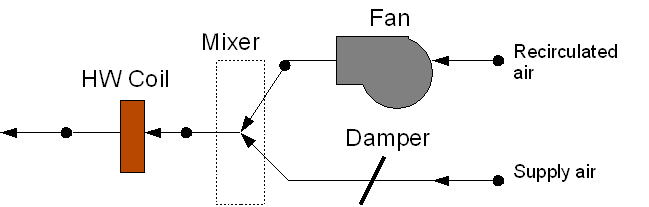
\includegraphics[width=0.9\textwidth, height=0.9\textheight, keepaspectratio=true]{media/image271.png}
\caption{Parallel PIU Terminal Unit \protect \label{fig:parallel-piu-terminal-unit}}
\end{figure}

\subsubsection{Inputs}\label{inputs-8-000}

\paragraph{Field: Name}\label{field-name-8-000}

A unique user assigned name for a particular~ parallel powered induction terminal unit. Any reference to this unit by another object will use this name.

\paragraph{Field: Availability Schedule Name}\label{field-availability-schedule-name-8}

The name of the schedule (ref: Schedule) that denotes whether the unit can run during a given time period. A schedule value greater than 0 (usually 1 is used) indicates that the unit can be on during the time period. A value less than or equal to 0 (usually 0 is used) denotes that the unit must be off for the time period. If this field is blank, the schedule has values of 1 for all time periods.

\paragraph{Field: Maximum Primary Air Flow Rate}\label{field-maximum-primary-air-flow-rate-1}

The maximum volumetric air flow rate of primary air through the unit in cubic meters per second. This is the primary air flow rate at full cooling load when the primary air damper is fully open.

\paragraph{Field: Maximum Secondary Air Flow Rate}\label{field-maximum-secondary-air-flow-rate}

The maximum volumetric air flow rate of secondary air through the unit in cubic meters per second. This flow rate can be any amount but is commonly less than the maximum primary air flow rate.

\paragraph{Field: Minimum Primary Air Flow Fraction}\label{field-minimum-primary-air-flow-fraction-1}

The minimum volumetric air flow rate of primary air through the unit expressed as a fraction of the maximum volumetric air flow rate of primary air. This input can be 0.0. When set to autosize and the Sizing:System's \emph{System Outdoor Air Method} associated with this terminal is set to Standard62.1SimplifiedProcedure, the autosized air flow fraction is calculated according to the ASHRAE Standard 62.1 Simplified Procedure.

\paragraph{Field: Fan On Flow Fraction}\label{field-fan-on-flow-fraction}

This is the fraction of the primary air flow at or below which the secondary fan turns on. In the parallel PIU the fan operation is intermittent. If the primary air flow is above this fraction of the maximum, the fan is off unless reheat is required. The fan will only operate if the Availability Schedule specified in the \hyperref[fanconstantvolume]{Fan:ConstantVolume} object (see Fan Name below) is >0 or when it is overridden by an availability manager (ref. \hyperref[availabilitymanagernightcycle]{AvailabilityManager:NightCycle} and others). If the availability manager status is CycleOnZoneFansOnly, then the fan will run only if there is a heating load.  If the status is CycleOn, then the fan will run according to the normal controls (low flow or reheat required).

\paragraph{Field: Supply Air Inlet Node Name}\label{field-supply-air-inlet-node-name-1}

The name of the HVAC system node from which the unit draws its primary or supply air

\paragraph{Field: Secondary Air Inlet Node Name}\label{field-secondary-air-inlet-node-name-1}

The name of the HVAC system node from which the unit draws its secondary or recirculated air. The unit can draw secondary air from its conditioned zone directly or from a return air plenum. Thus this node should be one of the zones exhaust air nodes (see \emph{Zone Air Exhaust Node} in \textbf{\hyperref[zonehvacequipmentconnections]{ZoneHVAC:EquipmentConnections}}) or an induced air node outlet of a return plenum (see \emph{Induced Air Outlet Node} in \textbf{\hyperref[airloophvacreturnplenum]{AirLoopHVAC:ReturnPlenum}}).

\paragraph{Field: Outlet Node Name}\label{field-outlet-node-name-1}

The name of the HVAC system node to which the unit sends its outlet air. This should be one of the inlet air nodes of the zone which is being served.

\paragraph{Field: Reheat Coil Air Inlet Node Name}\label{field-reheat-coil-air-inlet-node-name-1}

The name of the HVAC system node which is the inlet node of the unit's heating coil. This is also the outlet node of the unit's zone mixer.

\paragraph{Field: Zone Mixer Name}\label{field-zone-mixer-name-1}

The name of an zone mixer component (object: \hyperref[airloophvaczonemixer]{AirLoopHVAC:ZoneMixer}) which composes part of the unit. Note that some of the input for the mixer will duplicate input fields of the powered induction unit. One of the zone mixer inlet nodes should be the same as the supply air inlet node of the PIU; the other inlet node of the zone mixer should be the same as the air outlet node of the fan. The outlet node of the zone mixer should be the same as the inlet node of the heating coil.

\paragraph{Field: Fan Name}\label{field-fan-name-2}

The name of a fan component which composes part of the unit. Note that the fan's maximum flow rate should be the same as the maximum secondary air flow rate of the PIU and the type of fan object must be \hyperref[fansystemmodel]{Fan:SystemModel} or \hyperref[fanconstantvolume]{Fan:ConstantVolume}. The fan's inlet node should be the same as the PIU secondary air inlet node. The fan's outlet node should be the same as one of the zone mixer's inlet nodes. The secondary fan will run only when the Availability Schedule specified in the \hyperref[fanconstantvolume]{Fan:ConstantVolume} object is >0 or when it is overridden by an availability manager (ref. \hyperref[availabilitymanagernightcycle]{AvailabilityManager:NightCycle} and others). See description of fan controls under Fan On Flow Fraction above.

\paragraph{Field: Reheat Coil Object Type}\label{field-reheat-coil-object-type-4}

The type of coil in the PIU. The valid choices are:

\begin{itemize}
\item
  \hyperref[coilheatingwater]{Coil:Heating:Water}
\item
  \hyperref[coilheatingelectric]{Coil:Heating:Electric}
\item
  \hyperref[coilheatinggas-000]{Coil:Heating:Fuel}
\item
  \hyperref[coilheatingsteam]{Coil:Heating:Steam}
\end{itemize}

In other words, the PIU may have a hot water, gas, electric or steam reheat coil.

\paragraph{Field: Reheat Coil Name}\label{field-reheat-coil-name-4}

The name of the heating coil component which composes part of the unit. Note that the heating coil's air inlet node is the same as the zone mixer's outlet node and the heating coil's air outlet node is the same as the PIU outlet node.

\paragraph{Field: Maximum Hot Water or Steam Flow Rate}\label{field-maximum-hot-water-or-steam-flow-rate-5}

The maximum hot water or steam volumetric flow rate in m\(^{3}\)/s through the unit's heating coil. The steam volumetric flow rate is calculated at 100C and 101325 Pa. If the heating coil is gas or electric this field should be blank.

\paragraph{Field: Minimum Hot Water or Steam Flow Rate}\label{field-minimum-hot-water-or-steam-flow-rate-5}

The minimum hot water or steam volumetric flow rate in m\(^{3}\)/s through the unit's heating coil. The steam volumetric flow rate is calculated at 100C and 101325 Pa. If the heating coil is gas or electric this field should be blank.

\paragraph{Field: Convergence Tolerance}\label{field-convergence-tolerance-4}

The control tolerance for the unit heating output. The unit is controlled by matching the unit output to the zone demand. For units with water coils, the model must be numerically inverted to obtain a specified output. The convergence tolerance is the error tolerance used to terminate the numerical inversion procedure. Basically, this is the fraction:

\begin{equation}
\frac{{\left| {{Q_{PIU,out}} - {Q_{zone\;load}}} \right|}}{{{Q_{zone\;load}}}} \le ConvergenceTolerance
\end{equation}

For gas or electric heating coils, this input should be left blank. The default is 0.001.

An IDF example:

\begin{lstlisting}

AirTerminal:SingleDuct:ParallelPIU:Reheat,
            Zone 3 PPIU ATU,          ! Name of air terminal unit
            FanAndCoilAvailSched,     ! Availability schedule for series PIU ATU
            0.47,                     ! Maximum primary air flow rate through terminal unit
            0.375,                    ! Maximum secondary air flow rate through the terminal unit
            0.1,                      ! Minimum primary air flow rate (fraction of max)
            0.1,                      ! fan on flow fraction
            Zone 3 PIU Pri Air Inlet Node,   ! Air Terminal unit supply air inlet node
            Zone 3 PIU Sec Air Inlet Node,   ! Air Terminal unit secondary air inlet node
            Zone 3 PIU Air Outlet Node,      ! Air Terminal unit outlet node
            Zone 3 Reheat Air Inlet Node,    ! Reheat coil air inlet node (fan outlet node)
            Zone 3 PIU Mixer,                ! Air terminal unit mixer name
            Zone 3 PIU Fan,                  ! Air terminal unit fan name
            Coil:Heating:Water,              ! type of air terminal unit reheat coil
            Reheat Coil Zone 3,              ! name of air terminal unit reheat coil
            0.0013,                          ! Max Reheat Water Flow {Flow: m3/sec}
            0.0,                             ! Min Reheat Water Flow {Flow: m3/sec}
            0.001;                           ! Convergence tolerance
\end{lstlisting}

\subsubsection{Outputs}\label{outputs-8}

\begin{itemize}
\item
  HVAC,Average,Zone Air Terminal Primary Damper Position {[]}
\item
  HVAC,Average,Zone Air Terminal Heating Rate {[}W{]}
\item
  HVAC,Sum,Zone Air Terminal Heating Energy {[}J{]}
\item
  HVAC,Average,Zone Air Terminal Sensible Cooling Rate {[}W{]}
\item
  HVAC,Sum,Zone Air Terminal Sensible Cooling Energy {[}J{]}
\item
  HVAC,Average,Zone Air Terminal Outdoor Air Volume Flow Rate {[}m3/s{]}
\end{itemize}

\paragraph{Zone Air Terminal Primary Damper Position {[]}}\label{zone-air-terminal-parallel-piu-primary-damper-position}

This output is the variable air volume primary damper position required to meet the zone load. This is the average value over the frequency being reported. The damper position is defined as the terminal unit primary air mass flow rate divided by the terminal unit's maximum primary air mass flow rate.

\paragraph{Zone Air Terminal Heating Rate {[}W{]}}\label{zone-air-terminal-heating-rate-w-1}

This field reports the dry air heating addition rate of the parallel PIU terminal unit to the zone it is serving in Watts. This is determined by outlet and zone air conditions and the mass flow rate through the terminal unit.

\paragraph{Zone Air Terminal Heating Energy {[}J{]}}\label{zone-air-terminal-heating-energy-j-1}

This field reports the dry air heat addition of the parallel PIU terminal unit~ to the zone it is serving in Joules over the timestep being reported. This is determined by outlet and zone air conditions, the mass flow rate through the terminal unit, and the timestep.

\paragraph{Zone Air Terminal Sensible Cooling Rate {[}W{]}}\label{zone-air-terminal-sensible-cooling-rate-w-2}

This field reports the sensible heat extraction rate of the parallel PIU terminal unit from the zone it is serving in Watts. This is determined by the outlet and zone conditions and the mass flow rate through the terminal unit.

\paragraph{Zone Air Terminal Sensible Cooling Energy {[}J{]}}\label{zone-air-terminal-sensible-cooling-energy-j-2}

This field reports the dry air sensible heat extraction of the parallel PIU terminal unit from the zone it is serving in Joules over the timestep being reported. This is determined by outlet and zone air conditions, the mass flow rate through the terminal unit, and the timestep.

\paragraph{Zone Air Terminal Outdoor Air Volume Flow Rate {[}m3/s{]}}

This output is the amount of outdoor air entering the zone. This is the average value over the frequency being reported. The amount of outdoor air is defined as the terminal unit air volume flow rate multiplied by the fraction of outdoor air entering the air loop's outside air system.

\subsection{AirTerminal:SingleDuct:ConstantVolume:FourPipeInduction}\label{airterminalsingleductconstantvolumefourpipeinduction}

The four pipe induction terminal unit provides local hot water heating or chilled water cooling of induced zone air which then mixes with centrally conditioned supply air. An air conditioning system consisting of these terminal units is effectively a mixed central air / local hydronic system. The centrally conditioned air supplied to the induction terminal units is constant volume at quite high pressure. The central air is discharged through a nozzle in the terminal unit, inducing a flow of room air over a hydronic heating/cooling coil. The coil is connected either to a single inlet and outlet pipe (2 pipe unit) or to 2 inlets and 2 outlets (4 pipe unit). The heated or cooled induced air mixes with the centrally conditioned air before being discharged into the zone. The terminal units are usually expected to do only sensible cooling -- any dehumidification is done by the central air conditioning system.

The EnergyPlus model of the four pipe induction terminal unit is a compound component consisting of a hot water heating coil, a chilled water cooling coil, and an air mixer. The unit has two inlet air streams: the centrally conditioned supply air and the induced air from the zone. The induced air passes first through the heating coil, then through the cooling coil and finally through the mixer. The central supply air goes directly into the mixer. The water flow through the hot or cold water coil is varied to meet the zone air conditioning requirement. Note that EnergyPlus models the four pipe induction terminal unit as having separate heating and cooling coils whereas real units have only a single coil used for both heating and cooling. Note also that the four pipe induction unit model can be used to model a two pipe unit by simply adjusting the heating and cooling coil schedules so that the heating coil is off when the cooling coil is on and vice versa.

\subsubsection{Inputs}\label{inputs-9-000}

\paragraph{Field: Name}\label{field-name-9-000}

A unique user assigned name for a particular~ four pipe induction terminal unit. Any reference to this unit by another object will use this name.

\paragraph{Field: Availability Schedule Name}\label{field-availability-schedule-name-9}

The name of the schedule (ref: Schedule) that denotes whether the unit can run during a given time period. A schedule value greater than 0 (usually 1 is used) indicates that the unit can be on during the time period. A value less than or equal to 0 (usually 0 is used) denotes that the unit must be off for the time period. If this field is blank, the schedule has values of 1 for all time periods.

\paragraph{Field: Maximum Total Air Flow Rate}\label{field-maximum-total-air-flow-rate}

The maximum volumetric air flow rate discharged from the unit in cubic meters per second. Since this is a constant air volume unit, this is also the design, rated air flow rate of the unit. Note that this is the total discharge flow rate -- including both central supply and induced air.

\paragraph{Field: Induction Ratio}\label{field-induction-ratio}

The ratio of induced air flow rate to primary supply air flow rate. The default is 2.5 the supply air induces zone air flow at 2.5 times the primary supply air flow rate.

\paragraph{Field: Supply Air Inlet Node Name}\label{field-supply-air-inlet-node-name-2}

The name of the HVAC system node from which the unit draws its primary or supply air

\paragraph{Field: Induced Air Inlet Node Name}\label{field-induced-air-inlet-node-name}

The name of the HVAC system node from which the unit draws its secondary or recirculated air. This should be the same node as one of the zone exhaust nodes.

\paragraph{Field: Air Outlet Node Name}\label{field-air-outlet-node-name-6}

The name of the HVAC system node to which the unit sends its outlet air. This should be one of the inlet air nodes of the zone which is being served.

\paragraph{Field: Heating Coil Object Type}\label{field-heating-coil-object-type-1}

The type of heating coil in the terminal unit. The choices are:

\begin{itemize}
\tightlist
\item
  \hyperref[coilheatingwater]{Coil:Heating:Water}
\end{itemize}

In other words, the unit may have a hot water coil only.

\paragraph{Field: Heating Coil Name}\label{field-heating-coil-name-1}

The name of the heating coil component which composes part of the unit. Note that the heating coil's air inlet node is the same as the terminal unit's induced air inlet node. The heating coil's air outlet node is the same as the cooling coil's air inlet node.

\paragraph{Field: Maximum Hot Water Flow Rate}\label{field-maximum-hot-water-flow-rate}

The maximum hot water volumetric flow rate in m\(^{3}\)/sec through the unit's heating coil.

\paragraph{Field: Minimum Hot Water Flow Rate}\label{field-minimum-hot-water-flow-rate}

The minimum hot water volumetric flow rate in m\(^{3}\)/sec through the unit's heating coil.

\paragraph{Field: Heating Convergence Tolerance}\label{field-heating-convergence-tolerance}

The control tolerance for the unit heating output. The unit is controlled by matching the unit output to the zone demand. The model must be numerically inverted to obtain a specified output. The convergence tolerance is the error tolerance used to terminate the numerical inversion procedure. Basically, this is the fraction:

\begin{equation}
\frac{{\left| {{Q_{unit,out}} - {Q_{zone\;load}}} \right|}}{{{Q_{zone\;load}}}} \le ConvergenceTolerance
\end{equation}

The default is 0.001.

\paragraph{Field: Cooling Coil Object Type}\label{field-cooling-coil-object-type}

The type of cooling coil in the terminal unit. The choices are:

\begin{itemize}
\item
  \hyperref[coilcoolingwater]{Coil:Cooling:Water}
\item
  \hyperref[coilcoolingwaterdetailedgeometry]{Coil:Cooling:Water:DetailedGeometry}
\end{itemize}

In other words, the unit must use only the water cooling coils.

\paragraph{Field: Cooling Coil Name}\label{field-cooling-coil-name}

The name of the cooling coil component which composes part of the unit. Note that the cooling coil's air inlet node is the same as the heating coil's air outlet node. The cooling coil's air outlet node is the same as one of the zone mixer's inlets.

\paragraph{Field: Maximum Cold Water Flow Rate}\label{field-maximum-cold-water-flow-rate}

The maximum cold water volumetric flow rate in m\(^{3}\)/sec through the unit's cooling coil.

\paragraph{Field: Minimum Cold Water Flow Rate}\label{field-minimum-cold-water-flow-rate}

The minimum cold water volumetric flow rate in m\(^{3}\)/sec through the unit's cooling coil.

\paragraph{Field: Cooling Convergence Tolerance}\label{field-cooling-convergence-tolerance}

The control tolerance for the unit cooling output. The unit is controlled by matching the unit output to the zone demand. The model must be numerically inverted to obtain a specified output. The convergence tolerance is the error tolerance used to terminate the numerical inversion procedure. Basically, this is the fraction:

\begin{equation}
\frac{{\left| {{Q_{unit,out}} - {Q_{zone\;load}}} \right|}}{{{Q_{zone\;load}}}} \le ConvergenceTolerance
\end{equation}

The default is 0.001.

\paragraph{Field: Zone Mixer Name}\label{field-zone-mixer-name-2}

The name of an zone mixer component (object: \hyperref[airloophvaczonemixer]{AirLoopHVAC:ZoneMixer}) which composes part of the terminal unit. Note that some of the zone mixer's inputs will duplicate some of the terminal units's inputs. One of the zone mixer inlet nodes should be the same as the supply air inlet node of the terminal unit; the other inlet node of the zone mixer should be the same as the cooling coil air outlet node. The outlet node of the zone mixer should be the same as the outlet node of the terminal unit.

An IDF example:

\begin{lstlisting}

AirTerminal:SingleDuct:ConstantVolume:FourPipeInduction,
      SPACE2-1 FPIU,            !- Name of System
      ReheatCoilAvailSched,     !- System Availability schedule
      autosize,                 !- Maximum total air volume flow rate
      1.0,                      !- Induction ratio
      SPACE2-1 ATU Supply Node, !- Terminal unit supply air inlet node
      SPACE2-1 ATU Induc Node,  !- Terminal unit induced air inlet node
      SPACE2-1 In Node,         !- Terminal unit air outlet node
      COIL:Heating:Water,       !- Heating coil object
      SPACE2-1 HW Coil,         !- Heating coil name
      autosize,                 !- Max hot water flow
      0.0,                      !- Min hot water flow
      0.001,                    !- Heating Convergence Tolerance
      COIL:Cooling:Water,       !- Cooling coil object
      SPACE2-1 CW Coil,         !- Cooling coil name
      autosize,                 !- Max cold water flow
      0.0,                      !- Min cold water flow
      0.001,                    !- Cooling Convergence Tolerance
      SPACE2-1 ATU Mixer;       !- Zone mixer component name

  COIL:Heating:Water,
      SPACE2-1 HW Coil,        !- Coil Name
      ReheatCoilAvailSched,    !- Availability Schedule Name
      autosize,                !- UA of the Coil {W/K}
      autosize,                !- Max Water Flow Rate of Coil {m3/s}
      SPACE2-1 HW Coil Water In Node,  !- Coil_Water_Inlet_Node
      SPACE2-1 HW Coil Water Out Node, !- Coil_Water_Outlet_Node
      SPACE2-1 ATU Induc Node, !- Coil_Air_Inlet_Node
      SPACE2-1 HW Coil Air Out Node;   !- Coil_Air_Outlet_Node

  COIL:Cooling:Water,
      SPACE2-1 CW Coil,        !- Coil Name
      CWCoilAvailSched,        !- Availability Schedule
      autosize,                !- UA of the Coil
      autosize,                !- Max Water Flow Rate of Coil
      ,                        !- Leaving Relative Humidity of Coil
      SPACE2-1 CW Coil Water In Node,  !- Coil_Water_Inlet_Node
      SPACE2-1 CW Coil Water Out Node, !- Coil_Water_Outlet_Node
      SPACE2-1 HW Coil Air Out Node,   !- Coil_Air_Inlet_Node
      SPACE2-1 CW Coil Air Out Node;   !- Coil_Air_Outlet_Node

  AirLoopHVAC:ZoneMixer,
      SPACE2-1 ATU Mixer,              !- Mixer Name
      SPACE2-1 In Node,                !- Outlet_Node
      SPACE2-1 ATU Supply Node,        !- Inlet_Node_1
      SPACE2-1 CW Coil Air Out Node;   !- Inlet_Node_2
\end{lstlisting}

\subsubsection{Outputs}\label{outputs-9}

\begin{itemize}
\item
  HVAC,Average,Zone Air Terminal Outdoor Air Volume Flow Rate {[}m3/s{]}
\end{itemize}

\paragraph{Zone Air Terminal Outdoor Air Volume Flow Rate {[}m3/s{]}}

This output is the amount of outdoor air entering the zone. This is the average value over the frequency being reported. The amount of outdoor air is defined as the terminal unit air volume flow rate multiplied by the fraction of outdoor air entering the air loop's outside air system.

\subsection{AirTerminal:SingleDuct:ConstantVolume:FourPipeBeam}\label{airterminalsingleductconstantvolumefourpipebeam}

The four-pipe beam air terminal system is a mixed air-hydronic system. A central, single-duct forced-air system that supplies conditioned air to the zones. Chilled water circulates through ceiling-mounted fin-tube convector units to provide sensible cooling. Hot water circulates through the same convectors to provide heating. Water flow rate through the beam unit is varied to meet the zone sensible cooling or heating load. Any dehumidification is done by the central forced-air system. Thermodynamically, the cooled beam system resembles the four-pipe induction unit (\textbf{\hyperref[airterminalsingleductconstantvolumefourpipeinduction]{AirTerminal:SingleDuct:ConstantVolume:FourPipeInduction}}).

To model a typical four-pipe beam system the user will need to define a conventional central constant volume forced air system in order to deliver primary air to the beam. This central system (usually) provides outside air for ventilation. Primary air is normally delivered at a fixed temperature but could be reset by a schedule or using an outdoor air reset setpoint manager. On the supply side of this air loop there will be the usual central conditioning equipment: outside air mixer, fan, heating and cooling coil. On the zone equipment (demand) side of the loop, the four-pipe beams will be represented as air terminal units. Because the four-pipe beam can provide heating the system can avoid over-cooling zones during times of low load with cool primary air temperatures, similar to the action of a reheat coil in a VAV terminal. Therefore, it is not necessary to have additional zone equipment (such as baseboard heaters) to handle heating (or reheating) loads.

Although the four-pipe beam equipment in a zone is treated by the program as a single terminal unit, the actual installation will often have multiple beam units in each zone. In this model, it is only the total length of all the beams and the total air flow of all the units that are described, not the number of individual beam units.

If needed, the program (in its sizing calculation for the system) determines the total length of beams and primary supply air flow that is needed to meet the zone design loads. The four pipe beam air terminal sizing differs from other air terminals in that the primary supply air flow rate is sized using the entire performance model and the flow rate is not the direct result from the \hyperref[sizingzone]{Sizing:Zone} and \hyperref[sizingsystem]{Sizing:System} calculations. The flow rates will be somewhere between what an air terminal would size out using \emph{VentilationRequirement} or \emph{Sensible} in the \hyperref[sizingsystem]{Sizing:System} object (either setting can be used).

The model includes two different types of inputs for flow rates, ``design'' and ``rated \ldots{} per-meter.'' The design values are the actual sizes of the flow rates as viewed from the zone and central air handler (but before zone multipliers). The design values include all the individual beam units and their lengths. The rated per-meter values are used to characterize product performance at nominal rating conditions in such a way that it can be scaled to match the size of a zone. The performance characteristics at the rating point are not fixed in the program and can be entered by the user when they differ from default values. The rated per meter values are normalized by the linear dimensions of the beam and are generally obtained from product catalog data by dividing by the length of the beam. The rated primary air flow rate is assumed to be for sea level conditions while the design primary air flow rate is modeled for the location elevation above sea level.

\subsubsection{Inputs}\label{inputs-10-000}

\paragraph{Field: Name}\label{field-name-10-000}

A unique user-assigned name for a particular beam unit. Any reference to this unit by another object will use this name.

\paragraph{Field: Primary Air Availability Schedule Name}\label{field-primary-air-availability-schedule-name}

The name of the schedule that denotes whether the terminal unit is operating to provide primary air during a given time period. A schedule value greater than 0 (usually 1 is used) indicates that the unit is on and requesting primary air flow during the time period. A value less than or equal to 0 (usually 0 is used) denotes that the unit must be off for the time period. If this field is blank, the schedule has values of 1 for all time periods.

\paragraph{Field: Cooling Availability Schedule Name}\label{field-cooling-availability-schedule-name}

The name of the schedule that denotes whether the terminal unit is operating to provide cooling during a given time period. A schedule value greater than 0 (usually 1 is used) indicates that the unit is on and available for beam cooling during the time period. A value less than or equal to 0 (usually 0 is used) denotes that the unit must be off for the time period. If this field is blank, the schedule has values of 1 for all time periods. The primary air availability schedule named in the previous input field must have a value that is ``on'' during times that cooling is available.

\paragraph{Field: Heating Availability Schedule Name}\label{field-heating-availability-schedule-name}

The name of the schedule that denotes whether the terminal unit can operate to provide heating during a given time period. A schedule value greater than 0 (usually 1 is used) indicates that the unit is on and available for beam heating during the time period. A value less than or equal to 0 (usually 0 is used) denotes that the unit must be off for the time period. If this field is blank, the schedule has values of 1 for all time periods. The primary air availability schedule named in the input field above must have a value that is ``on'' during times that heating is available.

\paragraph{Field: Primary Air Inlet Node Name}\label{field-primary-air-inlet-node-name}

The name of the HVAC system air node from which the unit draws its primary air.

\paragraph{Field: Primary Air Outlet Node Name}\label{field-primary-air-outlet-node-name}

The name of the HVAC system air node that connects this terminal unit to the zone. The will be the same as one of the zone inlet nodes.

\paragraph{Field: Chilled Water Inlet Node Name}\label{field-chilled-water-inlet-node-name}

The name of the chilled water inlet node. If desired, the chilled water node connections can be omitted and the model will assume the intent is to model a two-pipe heating only beam.

\paragraph{Field: Chilled Water Outlet Node Name}\label{field-chilled-water-outlet-node-name}

The name of the chilled water outlet node.

\paragraph{Field: Design Primary Air Volume Flow Rate}\label{field-design-primary-air-volume-flow-rate}

This is the air flow rate (m3/s) of the primary air entering the air terminal unit from the central air handling unit. This input can be autosized.

\paragraph{Field: Design Chilled Water Volume Flow Rate}\label{field-design-chilled-water-volume-flow-rate}

The maximum chilled water flow rate (m3/s) for the unit(s) serving the entire zone. This input can be autosized based on the zone design load.

\paragraph{Field: Design Hot Water Volume Flow Rate}\label{field-design-hot-water-volume-flow-rate}

The maximum hot water flow rate (m3/s) for the unit(s) serving the entire zone. This input can be autosized based on the zone design load.

\paragraph{Field: Zone Total Beam Length (m)}\label{field-zone-total-beam-length-m}

The total length of all the beams in the zone (m). The real spaces may actually have a number of individual beam units of a specific length and this is the length of individual beams times the total number of beams in the thermal zone. It need not be an even multiple of actual unit's beam length but it can be if desired. This field is autosizable.

\paragraph{Field: Rated Primary Air Flow Rate per Beam Length (m3/s-m)}\label{field-rated-primary-air-flow-rate-per-beam-length-m3s-m}

This is the primary air volume flow rate at rating conditions divided by the length of the beam, in m3/s-m. This ``catalog'' value for volume flow rate input is converted to a mass flow rate using standard air density at sea level. This value will be used for sizing the design primary air volume flow rate if the total beam length is not also autosized. The default is 0.035 m3/s-m.

\paragraph{Field: Beam Rated Cooling Capacity per Beam Length (W/m)}\label{field-beam-rated-cooling-capacity-per-beam-length-wm}

This is the beam cooling capacity at rating conditions divided by the length of the beam, in W/m. This is only the cooling contributed by the chilled water circulating through the convector and is separate from any cooling (or heating) that may also be provided by the primary air. The default is 600 W/m.

\paragraph{Field: Beam Rated Cooling Room Air Chilled Water Temperature Difference (Delta C)}\label{field-beam-rated-cooling-room-air-chilled-water-temperature-difference-delta-c}

This input defines the value of the temperature difference between the room air and entering chilled water at the rating point, in delta Celsius. This ``catalog'' input helps to define the operating conditions that correspond with Rated Beam Cooling Capacity per Meter. It is used to normalize the independent variable in the input field called Beam Cooling Capacity Temperature Difference Modification Factor Curve or Table Name. The default is 10.0 delta C.

\paragraph{Field: Beam Rated Chilled Water Volume Flow Rate per Beam Length (m3/s-m)}\label{field-beam-rated-chilled-water-volume-flow-rate-per-beam-length-m3s-m}

This input defines the value of the chilled water flow rate per meter length of beam at the rating point, in m3/s-m. This input helps to define the operating conditions that correspond with Rated Beam Cooling Capacity per Meter. It is used to normalize the independent variable in the input field called Beam Cooling Capacity Chilled Water Flow Modification Factor Curve or Table Name. The default is 0.00005 m3/s-m.

\paragraph{Field: Beam Cooling Capacity Temperature Difference Modification Factor Curve Name}\label{field-beam-cooling-capacity-temperature-difference-modification-factor-curve-name}

This field is the name of a curve or table object that describes how the beam convector's cooling capacity varies as a function of the temperature difference between the zone air and the entering chilled water. The single independent variable is the ratio of the current simulation results for the difference between the air and entering water and the difference at the rating point. The result of the curve or table is multiplied by the rated capacity to adjust the cooling capacity.

\paragraph{Field: Beam Cooling Capacity Air Flow Modification Factor Curve Name}\label{field-beam-cooling-capacity-air-flow-modification-factor-curve-name}

This field is the name of a curve or table object that describes how the beam convector's cooling capacity varies as a function of the primary air flow rate. The single independent variable is the ratio of the current primary air flow rate and the primary air flow rate at the rating point. The result of the curve or table is multiplied by the rated capacity to adjust the cooling capacity. The factor is useful to adjust for a range of primary air flow rates that a given product can accommodate. However, since this is a constant volume air terminal, the modification does not typically vary during the simulation and the range of independent variable does not need to be all that broad in practice.

\paragraph{Field: Beam Cooling Capacity Chilled Water Flow Modification Factor Curve Name}\label{field-beam-cooling-capacity-chilled-water-flow-modification-factor-curve-name}

This field is the name of a curve or table object that describes how the beam convector's cooling capacity varies as a function of the water flow rate. The single independent variable is the ratio of the current fluid flow rate to the fluid flow rate at the rating point. The result of the curve or table is multiplied by the rated capacity to adjust the cooling capacity. The model will adjust the chilled water flow rate to vary cooling power to meet the zone load, so for control purposes, the range of the independent variable must include all the way down to zero flow, with zero capacity at zero flow.

\paragraph{Field: Beam Rated Heating Capacity per Beam Length (W/m)}\label{field-beam-rated-heating-capacity-per-beam-length-wm}

This is the beam heating capacity at rating conditions divided by the length of the beam, in W/m. This is only the heating contributed by the hot water circulating through the convector and is separate from any heating (or cooling) that may also be provided by the primary air. The default is 1.200 W/m.

\paragraph{Field: Beam Rated Heating Room Air Hot Water Temperature Difference (Delta C)}\label{field-beam-rated-heating-room-air-hot-water-temperature-difference-delta-c}

This input defines the value of the temperature difference between the entering hot water and the room air at the rating point, in delta Celsius. This input helps to define the operating conditions that correspond with Rated Beam Heating Capacity per Meter. It is used to normalize the independent variable in the input field called Beam Heating Capacity Temperature Difference Modification Factor Curve or Table Name. The default is 27.8 delta C.

\paragraph{Field: Beam Rated Hot Water Volume Flow Rate per Beam Length (m3/s-m)}\label{field-beam-rated-hot-water-volume-flow-rate-per-beam-length-m3s-m}

This input defines the value of the hot water flow rate per meter length of beam at the rating point, in m3/s/m, or more strictly m3/s-m. This input helps to define the operating conditions that correspond with Rated Beam Heating Capacity per Meter. It is used to normalize the independent variable in the input field called Beam Heating Capacity Hot Water Flow Modification Factor Curve or Table Name. The default is 0.00005 m3/s-m.

\paragraph{Field: Beam Heating Capacity Temperature Difference Modification Factor Curve Name}\label{field-beam-heating-capacity-temperature-difference-modification-factor-curve-name}

This field is the name of a curve or table object that describes how the beam convector's heating capacity varies as a function of the temperature difference between the entering hot water and the zone air. The single independent variable is the ratio of the current simulation results for the difference between the water and air and the difference at the rating point. The result of the curve or table is multiplied by the rated capacity to adjust the heating capacity.

\paragraph{Field: Beam Heating Capacity Air Flow Modification Factor Curve Name}\label{field-beam-heating-capacity-air-flow-modification-factor-curve-name}

This field is the name of a curve or table object that describes how the beam convectors heating capacity varies as a function of the primary air flow rate. The single independent variable is the ratio of the current primary air flow rate and the primary air flow rate at the rating point. The result of the curve or table is multiplied by the rated capacity to adjust the heating capacity. The factor is useful to adjust for a range of primary air rates that a given product can accommodate. However, since this is a constant volume air terminal, the modification does not typically vary during the simulation and the range of independent variable does not need to be all that broad in practice.

\paragraph{Field: Beam Heating Capacity Hot Water Flow Modification Factor Curve Name}\label{field-beam-heating-capacity-hot-water-flow-modification-factor-curve-name}

This field is the name of a curve or table object that describes how the beam convector's heating capacity varies as a function of the water flow rate. The single independent variable is the ratio of the current fluid flow rate to the fluid flow rate at the rating point. The result of the curve or table is multiplied by the rated capacity to adjust the heating capacity. The model will adjust the hot water flow rate to vary heating power to meet the zone load, so for control purposes, the range of the independent variable must include all the way down to zero flow, with zero capacity at zero flow.

An example input follows:

\begin{lstlisting}
  AirTerminal:SingleDuct:ConstantVolume:FourPipeBeam,
    Zone One 4pipe Beam, !- Name
    ALWAYS_ON , !- Primary Air Availability Schedule Name
    ALWAYS_ON , !- Cooling Availability Schedule Name
    ALWAYS_ON , !- Heating Availability Schedule Name
    Zone One 4pipe Beam Inlet Node Name , !- Primary Air Inlet Node Name
    Zone One 4pipe Beam Outlet Node Name , !- Primary Air Outlet Node Name
    Zone One 4pipe Beam CW Inlet Node , !- Chilled Water Inlet Node Name
    Zone One 4pipe Beam CW Outlet Node , !- Chilled Water Outlet Node Name
    AUTOSIZE , !- Design Primary Air Volume Flow Rate
    AUTOSIZE , !- Design Chilled Water Volume Flow Rate
    AUTOSIZE , !- Design Hot Water Volume Flow Rate
    AUTOSIZE , !- Zone Total Beam Length
    0.036 , !- Rated Primary Air Flow Rate per Beam Length
    597 , !- Rated Beam Cooling Capacity per Beam Length
    10.0 , !- Rated Cooling Room Air Chilled Water Temperature Difference
    5.2E-5 , !- Rated Chilled Water Volume Flow Rate per Beam Length
    CapModFuncOfTempDiff, !- Beam Cooling Capacity Temperature Difference Modification Factor Curve or Table Name
    CoolCapModFuncOfSAFlow, !- Beam Cooling Capacity Air Flow Modification Factor Curve or Table Name
    CapModFuncOfWaterFlow, !- Beam Cooling Capacity Chilled Water Flow Modification Factor Curve or Table Name
    1548 , !- Rated Beam Heating Capacity per Beam Length
    27.8, !- Rated Heating Room Air Hot Water Temperature Difference
    5.2E-5, !- Rated Hot Water Volume Flow Rate per Beam Length
    CapModFuncOfTempDiff, !- Beam Heating Capacity Temperature Difference Modification Factor Curve or Table Name
    HeatCapModFuncOfSAFlow, !- Beam Heating Capacity Air Flow Modification Factor Curve or Table Name
    CapModFuncOfWaterFlow; !- Beam Heating Capacity Hot Water Flow Modification Factor Curve or Table Name
\end{lstlisting}

\subsubsection{Outputs}\label{outputs-10}

\paragraph{Zone Air Terminal Beam Sensible Cooling Rate {[}W{]}}\label{zone-air-terminal-beam-sensible-cooling-rate-w}

\paragraph{Zone Air Terminal Beam Sensible Cooling Energy {[}J{]}}\label{zone-air-terminal-beam-sensible-cooling-energy-j}

These are the sensible cooling power and energy delivered by the beams to the zone, exclusive of any cooling or heating done by the primary air.

\paragraph{Zone Air Terminal Beam Sensible Heating Rate {[}W{]}}\label{zone-air-terminal-beam-sensible-heating-rate-w}

\paragraph{Zone Air Terminal Beam Sensible Heating Energy {[}J{]}}\label{zone-air-terminal-beam-sensible-heating-energy-j}

These are the sensible heating power and energy delivered by the beams to the zone, exclusive of any cooling or heating done by the primary air.

\paragraph{Zone Air Terminal Primary Air Sensible Cooling Rate {[}W{]}}\label{zone-air-terminal-primary-air-sensible-cooling-rate-w}

Sensible cooling by the primary air to the zone, exclusive of any cooling or heating done by the beams.

\paragraph{Zone Air Terminal Primary Air Sensible Cooling Energy {[}J{]}}\label{zone-air-terminal-primary-air-sensible-cooling-energy-j}

Sensible cooling by the primary air to the zone, exclusive of any cooling or heating done by the beams.

\paragraph{Zone Air Terminal Primary Air Sensible Heating Rate {[}W{]}}\label{zone-air-terminal-primary-air-sensible-heating-rate-w}

Heating by the primary air to the zone, exclusive of any cooling or heating done by the beams.

\paragraph{Zone Air Terminal Primary Air Sensible Heating Energy {[}J{]}}\label{zone-air-terminal-primary-air-sensible-heating-energy-j}

Heating by the primary air to the zone, exclusive of any cooling or heating done by the beams.

\paragraph{Zone Air Terminal Primary Air Flow Rate {[}m3/s{]}}\label{zone-air-terminal-primary-air-flow-rate-m3s}

Air flow rate from the central air handler into the zone in m3/s. Note that this does not include any of the secondary air flow that is induced by the convector and nozzle action (the model does not resolve secondary air flow rate and the result are not available).

\paragraph{Zone Air Terminal Outdoor Air Volume Flow Rate {[}m3/s{]}}

This output is the amount of outdoor air entering the zone. This is the average value over the frequency being reported. The amount of outdoor air is defined as the terminal unit air volume flow rate multiplied by the fraction of outdoor air entering the air loop's outside air system.

\subsection{AirTerminal:SingleDuct:ConstantVolume:CooledBeam}\label{airterminalsingleductconstantvolumecooledbeam}

The Cooled Beam system is a mixed air-hydronic system. A central, single-duct forced-air system supplies conditioned ventilation air to the zones. Sensible cooling is done by chilled water circulating through ceiling mounted cooled beam units. Chilled water flow rate through the cooled beam units is varied to meet the zone sensible cooling load. Any dehumidification is done by the central ventilation air system. Heating is usually accomplished with hot water radiators. Thermodynamically, the cooled beam system resembles the four-pipe induction unit.

To model a typical cooled beam system the user will need to define a conventional central constant volume forced air system. This system will normally be 100\% outside air delivered at a fixed supply temperature (which could be reset by schedule or by outside air temperature). On the supply side of this air loop there will be the usual central AC equipment: outside air mixer, fan, heating and cooling coil. On the zone equipment (demand) side of the loop, the chilled beams will be represented as terminal units. Additional zone equipment (such as baseboard heaters) will be needed to handle heating loads.

Although the cooled beam equipment in a zone is treated by the program as a single terminal unit, the actual installation will have multiple beams in each zone. The program (in its sizing calculation for the system) figures out how many beams of what length are needed to meet the zone design load.

\subsubsection{Inputs}\label{inputs-11-000}

\paragraph{Field: Name}\label{field-name-11-000}

A unique user assigned name for a particular chilled beam unit. Any reference to this unit by another object will use this name.

\paragraph{Field: Availability Schedule Name}\label{field-availability-schedule-name-10}

The name of the schedule (ref: Schedule) that denotes whether the unit can run during a given time period. A schedule value greater than 0 (usually 1 is used) indicates that the unit can be on during the time period. A value less than or equal to 0 (usually 0 is used) denotes that the unit must be off for the time period. If this field is blank, the schedule has values of 1 for all time periods.

\paragraph{Field: Cooled Beam Type}\label{field-cooled-beam-type}

Two types of units are modeled: \emph{Active} or \emph{Passive}. In the active unit, primary air is supplied through the beam, inducing some secondary zone air into contact with the coil. This unit acts as an active convector. The passive unit is simply a passive, finned convector. Primary air is supplied through a normal diffuser.

\paragraph{Field: Supply Air Inlet Node Name}\label{field-supply-air-inlet-node-name-3}

The name of the HVAC system node from which the unit draws its primary or supply air. Note that this field should be specified for both types of unit, even though supply air does not pass through the passive unit.

\paragraph{Field: Supply Air Outlet Node Name}\label{field-supply-air-outlet-node-name}

The name of the air node that connects this terminal unit to the zone. The will be the same as one of the zone inlet nodes. The name of this node must be entered even if the actual beams are passive and is not actually supplying air to the zone.

\paragraph{Field: Chilled Water Inlet Node Name}\label{field-chilled-water-inlet-node-name-1}

The name of the chilled water inlet node.

\paragraph{Field: Chilled Water Outlet Node Name}\label{field-chilled-water-outlet-node-name-1}

The name of the chilled water outlet node.

\paragraph{Field: Supply Air Volumetric Flow Rate}\label{field-supply-air-volumetric-flow-rate}

This is the air flow rate in cubic meters per second of the supply air entering the zone. This input would normally be autosized based on the ventilation requirement (see Zone Sizing).

\paragraph{Field: Maximum Total Chilled Water Volumetric Flow Rate}\label{field-maximum-total-chilled-water-volumetric-flow-rate}

The maximum chilled water flow rate (in cubic meters per second) for the unit. This input would normally be autosized based on the zone design load.

\paragraph{Field: Number of Beams}\label{field-number-of-beams}

The number of individual cooled beam units in the zone. Normally this unit would be autocalculated by the program based upon the previous field and the nominal flow rate for a single beam unit (set by the program to 0.07 kg/s).

\paragraph{Field: Beam Length}\label{field-beam-length}

The length of an individual beam in meters. Normally this will be autocalculated by the program based upon the number of beam units and the zone design sensible cooling load. 1 to 4 meters is a typical length range.

\paragraph{Field: Design Inlet Water Temperature}\label{field-design-inlet-water-temperature}

The nominal or design inlet water temperature in degrees Celsius. The default is 15°C.

\paragraph{Field: Design Outlet Water Temperature}\label{field-design-outlet-water-temperature}

The nominal or design outlet water temperature in degrees Celsius. The default is 17°C.

\emph{The following inputs are parameters used to characterize the performance of the chilled beam units. Values for a given unit can be obtained from the manufacturer. The parameters are used in the following equations.~~~~~}

\emph{P\(_{beam}\)} = \emph{A·K·DT~~~~~~~} ~~~~~~~~~~~~~~~~~~~~~~~ beam cooling output per unit length W/m

\emph{K = a·DT\(^{n1}\)·vr\(^{n2}\)·w\(^{n3}\)}~~~~~~~~~~~~~~~~~~~~~~~~~~~ coil heat transfer coefficient W/(m\(^{2}\)K)

\emph{vr = (q\(_{in}\)}/a\emph{\(_{0}\))·r\(_{air}\)}~~~~~~~~~~~~~~~~~~~~~~~~~~~~~~~~~ room air mass flow rate across coil kg/(m\(^{2}\)s)

\emph{q\(_{in}\) = K\(_{1}\)·DT\(^{n}\)+K\(_{in}\)·q\(_{pr}\)}~~~~~~~~~~~~~~~~ room air volumetric flow rate across coil per

unit length m\(^{3}\)/(s-m)

DT is the room air --water temperature difference (average water temperature is used) in degrees C.

w is the water velocity in m/s.

q\(_{pr}\) is the supply air flow rate per unit length m\(^{3}\)/(s-m)

\paragraph{Field: Coil Surface Area per Coil Length}\label{field-coil-surface-area-per-coil-length}

Surface area on the air side of the beam per unit beam length. The units are square meters per meter. The default is 5.422. This is \emph{A} in the above equations.

\paragraph{Field: Model Parameter a (a)}\label{field-model-parameter-a-a}

This is ain the above equations. The default is 15.3

\paragraph{Field: Model Parameter n1}\label{field-model-parameter-n1}

This is n1 in the above equations. The default is 0.

\paragraph{Field: Model Parameter n2}\label{field-model-parameter-n2}

This is n2 in the above equations. The default is 0.84.

\paragraph{Field: Model Parameter n3}\label{field-model-parameter-n3}

This is n3 in the above equations. The default is 0.12.

\paragraph{Field: Model Parameter a\(_{0}\) (a)}\label{field-model-parameter-aux5f0-a}

This is a\(_{0}\) in the above equations. It is the free area of the coil in plan view (for the air flow) per unit beam length. The units are square meters per meter. The default is 0.171.

\paragraph{Field: Model Parameter K\(_{1}\) (K1)}\label{field-model-parameter-kux5f1-k1}

This is K\(_{1}\) in the above equations. The default is 0.005.

\paragraph{Field: Model Parameter n}\label{field-model-parameter-n}

This is n in the above equations. The default is 0.4.

\paragraph{Field: Coefficient of Induction K\(_{in}\) (Kin)}\label{field-coefficient-of-induction-kux5fin-kin}

The coefficient of induction K\(_{in}\) in the above equations. The default is 2.0 for active beams and 0.0 for passive beams.

\paragraph{Field: Pipe Inside Diameter}\label{field-pipe-inside-diameter}

The water pipe inside diameter in meters. The default is 0.0145.

An example input is:

\begin{lstlisting}

  AirTerminal:SingleDuct:ConstantVolume:CooledBeam,
      SPACE2-1 CB,             !- Name
      CWCoilAvailSched,        !- Availability Schedule Name
      Active,                  !- Cooled Beam Type
      SPACE2-1 ATU Supply Node,!- Supply Air Inlet Node Name
      SPACE2-1 In Node,        !- Supply Air Outlet Node Name
      SPACE2-1 CW Coil Water In Node,  !- Chilled Water Inlet Node Name
      SPACE2-1 CW Coil Water Out Node, !- Chilled Water Outlet Node Name
      ,                        !- Supply Air Volumetric Flow Rate
      ,                   !- Maximum Total Chilled Water Volumetric Flow Rate
      ,                        !- Number of Beams
      ,                        !- Beam Length
      ,                        !- Design Inlet Water Temperature
      ,                        !- Design Outlet Water temperature
      ,                        !- Coil Surface Area per Coil Length
      ,                        !- Model Parameter a
      ,                        !- Model Parameter n1
      ,                        !- Model Parameter n2
     ,                        !- Model Parameter n3
      ,                        !- Model Parameter a0
      ,                        !- Model Parameter K1
      ,                        !- Model Parameter n
      ,                        !- Coefficient of Induction Kin
      ;                        !- Leaving Pipe Inside Diameter
\end{lstlisting}

\subsubsection{Outputs}\label{outputs-11}

\begin{itemize}
\item
  HVAC,Sum,Zone Air Terminal Beam Sensible Cooling Energy {[}J{]}
\item
  HVAC,Average,Zone Air Terminal Beam Sensible Cooling Rate {[}W{]}
\item
  HVAC,Sum, Zone Air Terminal Supply Air Sensible Cooling Energy {[}J{]}
\item
  HVAC,Average,Zone Air Terminal Supply Air Sensible Cooling Rate {[}W{]}
\item
  HVAC,Sum,Zone Air Terminal Supply Air Sensible Heating Energy {[}J{]}
\item
  HVAC,Average,Zone Air Terminal Supply Air Sensible Heating Rate {[}W{]}
\item
  HVAC,Sum,Zone Air Terminal Beam Chilled Water Energy {[}J{]}
\item
  HVAC,Average,Zone Air Terminal Outdoor Air Volume Flow Rate {[}m3/s{]}
\end{itemize}

\paragraph{Zone Air Terminal Beam Sensible Cooling Rate {[}W{]}}\label{zone-air-terminal-beam-sensible-cooling-rate-w-1}

Sensible cooling by the beams in the zone, exclusive of any cooling or heating done by the supply air.

\paragraph{Zone Air Terminal Beam Sensible Cooling Energy {[}J{]}}\label{zone-air-terminal-beam-sensible-cooling-energy-j-1}

Sensible cooling by the beams in the zone, exclusive of any cooling or heating done by the supply air.

\paragraph{Zone Air Terminal Supply Air Sensible Cooling Rate {[}W{]}}\label{zone-air-terminal-supply-air-sensible-cooling-rate-w}

Sensible cooling by the supply air to the zone, exclusive of any cooling done by the beams.

\paragraph{Zone Air Terminal Supply Air Sensible Cooling Energy {[}J{]}}\label{zone-air-terminal-supply-air-sensible-cooling-energy-j}

Sensible cooling by the supply air to the zone, exclusive of any cooling done by the beams.

\paragraph{Zone Air Terminal Supply Air Sensible Heating Rate {[}W{]}}\label{zone-air-terminal-supply-air-sensible-heating-rate-w}

Heating by the supply air to the zone, exclusive of any cooling done by the beams.

\paragraph{Zone Air Terminal Supply Air Sensible Heating Energy {[}J{]}}\label{zone-air-terminal-supply-air-sensible-heating-energy-j}

Heating by the supply air to the zone, exclusive of any cooling done by the beams.

\paragraph{Zone Air Terminal Beam Chilled Water Energy {[}J{]}}\label{zone-air-terminal-beam-chilled-water-energy-j}

The heat transfer energy for the chilled water serving the beams, in Joules.

\paragraph{Zone Air Terminal Outdoor Air Volume Flow Rate {[}m3/s{]}}

This output is the amount of outdoor air entering the zone. This is the average value over the frequency being reported. The amount of outdoor air is defined as the terminal unit air volume flow rate multiplied by the fraction of outdoor air entering the air loop's outside air system.

\subsection{AirTerminal:SingleDuct:Mixer}\label{airterminalsingleductmixer}

The air terminal mixer provides a means of supplying central system air either to air inlet or supply side of a ZoneHVAC equipment such as a four pipe fan coil. Normally the central air would be ventilation air from a dedicated outside air system (DOAS).

This terminal mixer object mixes conditioned outdoor air (primary air) from DOAS air loop and recirculating (secondary air) and deliver it either to inlet or supply side of a local ZoneHVAC equipment. The terminal mixer can be connected either to the inlet or supply side of the local ZoneHVAC equipment and the connection type is specified in the input field \textit{Mixer Connection Type}. If the AirTerminal:SingleDuct:Mixer object is connected to the supply side, a mix of conditioned outdoor air from a central dedicated outdoor air system (DOAS) with conditioned recirculation air from the local ZoneHVAC equipment is supplied as a single stream to the conditioned zone at its inlet node. If the AirTerminal:SingleDuct:Mixer object is connected to the inlet side, a mix of outdoor air from the a central dedicated outdoor air system (DOAS) with un-conditioned recirculation air from a zone exhaust node is supplied to the ZoneHVAC equipment inlet node. The mixer model will sum the two air streams and average the air properties. The AirTerminal:SingleDuct:Mixer is used with:

\begin{itemize}
\setlength{\parskip}{0pt}
\setlength{\itemsep}{0pt plus 2pt}
\item \hyperref[zonehvacfourpipefancoil]{ZoneHVAC:FourPipeFanCoil}
\item \hyperref[zonehvacwatertoairheatpump]{ZoneHVAC:WaterToAirHeatPump}
\item \hyperref[zonehvacpackagedterminalairconditioner]{ZoneHVAC:PackagedTerminalAirConditioner}
\item \hyperref[zonehvacpackagedterminalheatpump]{ZoneHVAC:PackagedTerminalHeatPump}
\item \hyperref[zonehvacterminalunitvariablerefrigerantflow]{ZoneHVAC:TerminalUnit:VariableRefrigerantFlow}
\item \hyperref[zonehvacunitventilator]{ZoneHVAC:UnitVentilator}
\item \hyperref[airloophvacunitarysystem]{AirLoopHVAC:UnitarySystem}
\end{itemize}


The \hyperref[airloophvacunitarysystem]{AirLoopHVAC:UnitarySystem} object must be specified as a ZoneHVAC equipment. Since the ZoneHVAC equipment gets the outdoor air or ventilation air from central dedicated OA system, the design outdoor air flow rate input fields in the ZoneHVAC equipment are set to zero and the \hyperref[outdoorairmixer]{OutdoorAir:Mixer} object type and object name input fields are left blank.

\begin{figure}[hbtp] % fig 108
\centering
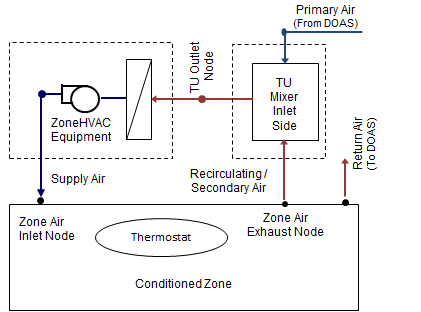
\includegraphics[width=0.9\textwidth, height=0.9\textheight, keepaspectratio=true]{media/image275.png}
\caption{Inlet Side Mixer Air Terminal Unit with ZoneHVAC Equipment \protect \label{fig:inlet-side-mixer-air-terminal-unit-with-ZoneHVAC-equipment}}
\end{figure}
\begin{figure}[hbtp] % fig 109
\centering
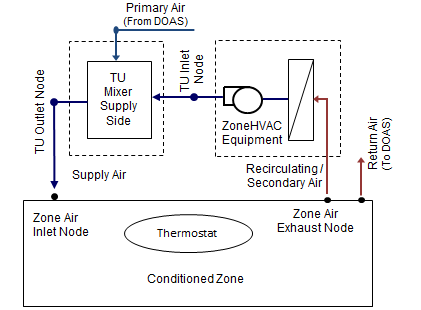
\includegraphics[width=0.9\textwidth, height=0.9\textheight, keepaspectratio=true]{media/image276.png}
\caption{Supply Side Mixer Air Terminal Unit with ZoneHVAC equipment \protect \label{fig:supply-side-mixer-air-terminal-unit-with-ZoneHVAC-equipment}}
\end{figure}



\subsubsection{Inputs}\label{inputs-12-000}

\paragraph{Field: Name}\label{field-name-12}

A unique user assigned name for a particular terminal mixer unit. Any reference to this unit by another object will use this name.

\paragraph{Field: ZoneHVAC Unit Object Type}\label{field-zonehvac-unit-object-type}

The type of ZoneHVAC equipment to which this terminal mixer will be connected. This is a choice input field.
Valid ZoneHVAC choices are:
\begin{itemize}
\setlength{\parskip}{0pt}
\setlength{\itemsep}{0pt plus 1pt}
\item \hyperref[zonehvacfourpipefancoil]{ZoneHVAC:FourPipeFanCoil}
\item \hyperref[zonehvacwatertoairheatpump]{ZoneHVAC:WaterToAirHeatPump}
\item \hyperref[zonehvacpackagedterminalairconditioner]{ZoneHVAC:PackagedTerminalAirConditioner}
\item \hyperref[zonehvacpackagedterminalheatpump]{ZoneHVAC:PackagedTerminalHeatPump}
\item \hyperref[zonehvacterminalunitvariablerefrigerantflow]{ZoneHVAC:TerminalUnit:VariableRefrigerantFlow}
\item \hyperref[zonehvacunitventilator]{ZoneHVAC:UnitVentilator}
\item \hyperref[airloophvacunitarysystem]{AirLoopHVAC:UnitarySystem}
\end{itemize}

\paragraph{Field: ZoneHVAC Unit Object Name}\label{field-zonehvac-unit-object-name}

The name of ZoneHVAC equipment to which this mixer will be connected.

\paragraph{Field: Mixer Outlet Node Name}\label{field-mixer-outlet-node-name}

The outlet air node name of the mixer. This will be an inlet air node name of the conditioned zone if the connection type specified in the input field \textit{Mixer Connection Type} below is \textbf{SupplySide}, or else this will be the inlet air node name of the ZoneHVAC equipment if the connection type in the input field \textit{Mixer Connection Type} below is \textbf{InletSide}.

\paragraph{Field: Mixer Primary Air Inlet Node Name}\label{field-mixer-primary-air-inlet-node-name}

The primary air (treated outdoor air) inlet node name of the mixer. This will be the outlet air node name of an \hyperref[airloophvaczonesplitter]{AirLoopHVAC:ZoneSplitter} or \hyperref[airloophvacsupplyplenum]{AirLoopHVAC:SupplyPlenum}, providing the connection to the DOAS system.

\paragraph{Field: Mixer Secondary Air Inlet Node Name}\label{field-mixer-secondary-air-inlet-node-name}

The secondary air (recirculating air) inlet node name of the mixer. This will be the outlet air node name of the ZoneHVAC equipment if the connection type in the input field \textit{Mixer Connection Type} below is \textbf{SupplySide}, or else this will be either an exhaust air node name of the conditioned zone (Ref. \hyperref[zonehvacequipmentconnections]{ZoneHVAC:EquipmentConnections} to draw air from a zone directly or an induced air outlet node (Ref. \hyperref[airloophvacreturnplenum]{AirLoopHVAC:ReturnPlenum}) to draw air from a return plenum when the zone return node is connected to a return plenum.  The induced air outlet node will be the outlet air node name when the mixer connection type is SupplySide. If the mixer connection type is InletSide, then the induced air outlet node will be the mixer secondary air inlet node.

\paragraph{Field: Mixer Connection Type}\label{field-mixer-connection-type}

This input field allows user to specify the mixer connection type. Valid choices are \textbf{InletSide} or \textbf{SupplySide}. This is a required input field. If the mixer connection type selected is \textbf{InletSide}, then the mixer is connected on the inlet side of the ZoneHVAC equipment, or else if the mixer connection type selected is \textbf{SupplySide}, then the mixer is connected at the outlet side of the ZoneHVAC equipment.\\

\paragraph{Field: Design Specification Outdoor Air Object Name}\label{field-DSOA-object-name}

This field allows modifying the behavior of this air terminal so that it is modulated to supply the required outdoor air to the zone.  This field is optional. When the name of an \hyperref[designspecificationoutdoorair]{DesignSpecification:OutdoorAir} or \hyperref[designspecificationoutdoorairspacelist]{DesignSpecification:OutdoorAir:SpaceList} object is entered, the model is changed to adjust the flow rate to provide the volume of outdoor air described by that object.  This feature allows modeling demand controlled ventilation on a zone-by-zone basis using the Outdoor Air Flow per Person rate (specified in the \hyperref[designspecificationoutdoorair]{DesignSpecification:OutdoorAir} object) and the number of occupants (specified in the \hyperref[people]{People} object schedules).  If the outdoor air fraction of the supply air is 1.0, as for a dedicated outdoor air system, the air flow rate will match the outdoor air requirement.  When the outdoor air fraction is less than 1.0, as for a recirculating air system, the terminal air flow will be modulated upward to account for the increased total air flow needed to provide the required flow rate of outdoor air.   The total air flow rate will not exceed the Maximum Air Flow Rate specified above. The volume flow rate is converted to mass flow rate using the standard density of air at Pressure = 101325 Pa, Temperature = 20C, and Humidity Ratio = 0.0.

\paragraph{Field: Per Person Ventilation Rate Mode}

This field specifies how the outdoor air ventilation rates are calculated when based on a rate per person.~ It can be either based on the current number of people as affected by time-varying occupancy schedules, or on the constant value for the maximum number of people.~~ Enter the key CurrentOccupancy for the former and DesignOccupancy for the later.

An IDF examples for InletSide and SupplySide connection type:

\begin{lstlisting}

AirTerminal:SingleDuct:Mixer,
      SPACE2-1 DOAS Air Terminal,  !- Name
      ZoneHVAC:FourPipeFanCoil,    !- ZoneHVAC Unit Object Type
      SPACE2-1 Fan Coil,           !- ZoneHVAC Unit Object Name
      SPACE2-1 Fan Coil Inlet,     !- Mixer Outlet Node Name
      SPACE2-1 ATM Primary Inlet,  !- Mixer Primary Air Inlet Node Name
      SPACE2-1 ATM Secondary Inlet,!- Mixer Secondary Air Inlet Node Name
      InletSide;                   !- Mixer Connection Type
\end{lstlisting}

\begin{lstlisting}

AirTerminal:SingleDuct:Mixer,
      SPACE1-1 DOAS Air Terminal, !- Name
      ZoneHVAC:FourPipeFanCoil,   !- ZoneHVAC Unit Object Type
      SPACE1-1 Fan Coil,          !- ZoneHVAC Unit Object Name
      SPACE1-1 Supply Inlet,      !- Mixer Outlet Node Name
      SPACE1-1 ATM Primary Inlet, !- Mixer Primary Air Inlet Node Name
      SPACE1-1 Fan Coil Outlet,   !- Mixer Secondary Air Inlet Node Name
      SupplySide;                 !- Mixer Connection Type
\end{lstlisting}

\subsection{AirTerminal:DualDuct:ConstantVolume}\label{airterminaldualductconstantvolume}

The AirTerminal:DualDuct:ConstantVolume simulation or the typical Multizone is described by this Air Distribution Unit (ADU). Multizone systems condition all the air in a central apparatus and distribute it to the conditioned zones through two parallel ducts. One duct carries cold air and the other warm air, providing air sources for both heating and cooling at all times. In each conditioned zone, a mixing valve responsive to a room thermostat mixes the warm and cold air in proper proportions to satisfy the prevailing heating or cooling load of the space. The Multizone ADU is the specific component that leads to the zone containing the mixer and the mixing damper and then connecting to the zone. The total airflow to each room is kept constant while the proportion of hot air to cold air is adjusted to maintain the temperature in each zone at the desired level.

\subsubsection{Inputs}\label{inputs-14-000}

\paragraph{Field: Name}\label{field-name-14}

Unique name for the Multizone ADU.

\paragraph{Field: Availability Schedule Name}\label{field-availability-schedule-name-11}

Schedule that this component will operate or is available to operate for a given time period. A schedule value greater than 0 (usually 1 is used) indicates that the component can be on during the time period. A value less than or equal to 0 (usually 0 is used) denotes that the component must be off for the time period. If this field is blank, the schedule has values of 1 for all time periods.

\paragraph{Field: Air Outlet Node Name}\label{field-air-outlet-node-name-7}

The outlet node from the ADU to the zone.

\paragraph{Field: Hot Air Inlet Node Name}\label{field-hot-air-inlet-node-name}

The air-inlet node name that connects the hot air splitter to the individual zone ADU.

\paragraph{Field: Cold Air Inlet Node Name}\label{field-cold-air-inlet-node-name}

The air-inlet node name that connects the cold air splitter to the individual zone ADU.

\paragraph{Field: Maximum Air Flow Rate}\label{field-maximum-air-flow-rate-7}

The design constant volume flow rate~ (m\(^{3}\)/sec) specified for that Multizone ADU.

An IDF example:

\begin{lstlisting}

AirTerminal:DualDuct:ConstantVolume,
      Zone2MixDamp,  !- Name
      FanAndCoilAvailSched,  !- Availability Schedule
      Zone 2 Dual Duct Outlet,  !- Unit Air Outlet Node
      Zone 2 Dual Duct Hot Inlet,  !- Unit Hot Air Inlet Node
      Zone 2 Dual Duct Cold Inlet,  !- Unit Cold Air Inlet Node
      0.36;  !- Max Air Flow Rate {m3/s}
\end{lstlisting}

\subsubsection{Outputs}\label{outputs-12}

\begin{itemize}
\item
  HVAC,Average,Zone Air Terminal Cold Supply Duct Damper Position {[]}
\item
  HVAC,Average,Zone Air Terminal Hot Supply Duct Damper Position {[]}
\end{itemize}

\paragraph{Zone Air Terminal Cold Supply Duct Damper Position}\label{zone-air-terminal-cold-supply-duct-damper-position}

This output is the damper position of the cold air stream in a dual duct air terminal. This is the average value over the frequency being reported. The damper position is defined as the terminal unit cold air mass flow rate divided by the terminal unit's maximum cold air mass flow rate. This output is dimensionless and ranges from 0.0 to 1.0.

\paragraph{Zone Air Terminal Hot Supply Duct Damper Position}\label{zone-air-terminal-hot-supply-duct-damper-position}

This output is the damper position of the hot air stream in a dual duct air terminal. This is the average value over the frequency being reported. The damper position is defined as the terminal unit hot air mass flow rate divided by the terminal unit's maximum hot air mass flow rate. This output is dimensionless and ranges from 0.0 to 1.0.

\subsection{AirTerminal:DualDuct:VAV}\label{airterminaldualductvav}

AirTerminal:DualDuct:VAV (i.e., Dual duct variable air volume (DDVAV)) systems are used to obtain zone temperature control by mixing the cold and warm air in various volume combinations. The fan is sized for the anticipated maximum coincident hot or cold volume, not the sum of the instantaneous peaks. This system has an advantage of a true single path VAV system, except for warm port leakage. When cold air is modulated for control before mixing, it operates similar to the VAV induction when mixing occurs without hot deck reheat. It is similar to a reheat system when mixing occurs while the hot deck is using the reheat coil. It uses more energy than a true VAV system, but less than a constant volume dual duct system.

The zone minimum supply air flow can be further adjusted using scheduled fraction values specified in the field \textit{Minimum Air Flow Turndown Schedule Name}.

\subsubsection{Inputs}\label{inputs-15-000}

\paragraph{Field: Name}\label{field-name-15}

Unique name for the AirTerminal:DualDuct:VAV Air Distribution Unit (ADU).

\paragraph{Field: Availability Schedule Name}\label{field-availability-schedule-name-12}

Schedule that this component will operate or is available to operate for a given time period. A schedule value greater than 0 (usually 1 is used) indicates that the component can be on during the time period. A value less than or equal to 0 (usually 0 is used) denotes that the component must be off for the time period. If this field is blank, the schedule has values of 1 for all time periods.

\paragraph{Field: Air Outlet Node Name}\label{field-air-outlet-node-name-8}

The outlet node from the ADU to the zone.

\paragraph{Field: Hot Air Inlet Node Name}\label{field-hot-air-inlet-node-name-1}

The air-inlet node name that connects the hot air splitter to the individual zone ADU.

\paragraph{Field: Cold Air Inlet Node Name}\label{field-cold-air-inlet-node-name-1}

The air-inlet node name that connects the cold air splitter to the individual zone ADU.

\paragraph{Field: Maximum Damper Air Flow Rate}\label{field-maximum-damper-air-flow-rate}

The design maximum volume flow rate~ (m\(^{3}\)/sec) specified for DDVAV ADU.

\paragraph{Field: Zone Minimum Air Flow Fraction}\label{field-zone-minimum-air-flow-fraction-3}

The minimum flow rate to the zone while the system is operating, specified as a fraction of the Max Damper Air Flow Rate. The minimum zone fraction is normally specified to meet the minimum ventilation requirement for the occupants.

\paragraph{Field: Design Specification Outdoor Air Object Name}\label{field-design-specification-outdoor-air-object-name-2}

This alpha field specifies the name of a \hyperref[designspecificationoutdoorair]{DesignSpecification:OutdoorAir} or \hyperref[designspecificationoutdoorairspacelist]{DesignSpecification:OutdoorAir:SpaceList} object. When this field is used, the terminal unit will increase flow as needed to meet this outdoor air requirement. If Outdoor Air Flow per Person is non-zero, then the outdoor air requirement will be computed based on the current number of occupants in the zone. At no time will the supply air flow rate exceed the value for Maximum Air Flow Rate. If this field is blank, then the terminal unit will not be controlled for outdoor air flow. See documentation for the zone HVAC outdoor air object for further information (Ref \hyperref[designspecificationoutdoorair]{DesignSpecification:OutdoorAir}).

\paragraph{Field: Minimum Air Flow Turndown Schedule Name}

This field adjusts \textit{Zone Minimum Air Flow Fraction} by multiplying it using this schedule. Schedule values are fractions, 0.0 to 1.0. This field adjusts the minimum airflow turndown value below the zone design minimum air flow and is intended for use with ASHRAE Standard 170. This field can also be used to adjust the design minimum air flow sizing calculation by applying a desired fraction values to summer and winter design days turndown schedule. If this field is left blank, then the turndown minimum air flow fraction value is set to 1 and the VAV air terminal uses the fixed fraction specified in in the field \textit{Zone Minimum Air Flow Fraction}.


An IDF example:

\begin{lstlisting}

  AirTerminal:DualDuct:VAV,
      Zone1MixDamp,            !- Name
      FanAndCoilAvailSched,    !- Availability Schedule Name
      Zone 1 Dual Duct Outlet, !- Air Outlet Node Name
      Zone 1 Dual Duct Hot Inlet,  !- Hot Air Inlet Node Name
      Zone 1 Dual Duct Cold Inlet,  !- Cold Air Inlet Node Name
      autosize,                !- Maximum Air Flow Rate {m3/s}
      0.1,                     !- Zone Minimum Air Flow Fraction
      ZoneMinOARequirements,   !- Design Specification Outdoor Air Object Name
      TurndownMinAirFlowSch;   !- Minimum Air Flow Turndown Schedule Name

  ! Outdoor air specification should be consistent with Sizing:Zone object inputs.
    DesignSpecification:OutdoorAir,
      ZoneMinOARequirements,    !- Name
      Sum,                      !- Outdoor Air Method
      0.00944,                  !- Outdoor Air Flow per Person {m3/s}
      0.000508,                 !- Outdoor Air Flow per Zone Floor Area {m3/s-m2}
      ,                         !- Outdoor Air Flow per Zone
      ,                         !- Outdoor Air Flow Air Changes per Hour
      Min OARequirements Sched; !- Outdoor Air Flow Rate Fraction Schedule Name

    Schedule:Compact,
      Min OARequirements Sched,  !- Name
      Any Number,                !- Schedule Type Limits Name
      Through: 12/31,            !- Field 1
      For: Weekdays SummerDesignDay WinterDesignDay, !- Field 2
      Until: 24:00,1.0,          !- Field 7
      For: AllOtherDays,         !- Field 9
      Until: 24:00,0.25;         !- Field 10

    Schedule:Compact,
      TurndownMinAirFlowSch,   !- Name
      Fraction,                !- Schedule Type Limits Name
      Through: 12/31,          !- Field 1
      For: Weekdays,           !- Field 2
      Until: 7:00,0.50,        !- Field 3
      Until: 17:00,0.75,       !- Field 4
      Until: 24:00,0.50,       !- Field 5
      For: SummerDesignDay WinterDesignDay, !- Field 6
      Until: 24:00,1.0,        !- Field 7
      For: Weekends Holidays CustomDay1 CustomDay2, !- Field 8
      Until: 24:00,0.25;       !- Field 9
\end{lstlisting}

\subsubsection{Outputs}\label{outputs-13}

\begin{itemize}
\item
  HVAC,Average,Zone Air Terminal Cold Supply Duct Damper Position {[]}
\item
  HVAC,Average,Zone Air Terminal Hot Supply Duct Damper Position {[]}
\item
  HVAC,Average,Zone Air Terminal Outdoor Air Volume Flow Rate {[}m3/s{]}
\end{itemize}

\paragraph{Zone Air Terminal Cold Supply Duct Damper Position {[]}}\label{zone-air-terminal-cold-supply-duct-damper-position-1}

This output is the damper position of the cold air stream in a dual duct air terminal. This is the average value over the frequency being reported. The damper position is defined as the terminal unit cold air mass flow rate divided by the terminal unit's maximum cold air mass flow rate.

\paragraph{Zone Air Terminal Hot Supply Duct Damper Position {[]}}\label{zone-air-terminal-hot-supply-duct-damper-position-1}

This output is the damper position of the hot air stream in a dual duct air terminal. This is the average value over the frequency being reported. The damper position is defined as the terminal unit hot air mass flow rate divided by the terminal unit's maximum hot air mass flow rate.

\paragraph{Zone Air Terminal Outdoor Air Volume Flow Rate {[}m3/s{]}}

This output is the amount of outdoor air entering the zone. This is the average value over the frequency being reported. The amount of outdoor air is defined as the terminal unit air volume flow rate multiplied by the fraction of outdoor air entering the air loop's outdoor air system.

\subsection{AirTerminal:DualDuct:VAV:OutdoorAir}\label{airterminaldualductvavoutdoorair}

AirTerminal:DualDuct:VAV:OutdoorAir provides a model for a type of dual duct air system in which one duct provides outdoor air ventilation and the other provides VAV cooling.~ The Outdoor Air stream and the Recirculated Air stream are conditioned and supplied through separate air streams as part of a centralized dedicated outdoor air~ (DOAS) distribution system. The dual duct arrangement allows the ventilation air to be controlled separately using schedules or occupancy demand while the recirculated air is controlled to meet the dry-bulb zone temperature setpoint. The two airstreams remain decoupled until the terminal box where they are mixed. The terminal unit is meant for systems regulating outdoor air based only on demand control or code minimum settings and not on economizer operation.

This air terminal does not have heating coils and is not configured for conditions zones that need heat. Additional ZoneHVAC equipment, such as baseboards or fan coil units, are needed to provide heating to the zone when using this air terminal.

Although this air terminal is primarily for dual duct system, it is allowed to use just the outdoor air side in a single duct system. This can be useful for modeling single duct DOAS when the required volume of outdoor air varies over time.

\subsubsection{Inputs}\label{inputs-16-000}

\paragraph{Field: Name}\label{field-name-16}

Unique name for the AirTerminal:DualDuct:VAV:OutdoorAir Air Distribution Unit (ADU).

\paragraph{Field: Availability Schedule Name}\label{field-availability-schedule-name-13}

Schedule that this component will operate or is available to operate for a given time period. A schedule value greater than 0 (usually 1 is used) indicates that the component can be on during the time period. A value less than or equal to 0 (usually 0 is used) denotes that the component must be off for the time period. If this field is blank, the schedule has values of 1 for all time periods.

\paragraph{Field: Air Outlet Node Name}\label{field-air-outlet-node-name-9}

The outlet node of the terminal unit.~ This is the node leaving the unit and serving as the inlet to the zone. It is for the mixed flow leaving from both of the inlet node.

\paragraph{Field: Outdoor Air Inlet Node Name}\label{field-outdoor-air-inlet-node-name}

The inlet node of the Outdoor Air (OA) stream deck of the Dual Duct system.

\paragraph{Field: Recirculated Air Inlet Node Name}\label{field-recirculated-air-inlet-node-name}

The inlet node of the Recirculated Air (RA) stream deck of the Dual Duct system. ~This input is optional. If no node name is entered here, then the recirculation duct is disabled and the model functions as a single duct terminal and no second cooling deck is needed.

\paragraph{Field: Maximum Zone Total Airflow Rate}\label{field-maximum-zone-total-airflow-rate}

Max total airflow rate (in m3/s) at the terminal unit outlet including both the Outdoor Air stream and the Recirculated stream.~ Can be autosized based on the Design Outdoor Airflow Rate and the zone thermal cooling load.~ The autosized flow rate will be the sum of the maximum outdoor air requirement and the flow for cooling. ~When autosizing, this maximum and the individual inlet flow rate sizes are reported to the eio file.

\paragraph{Field: Design Specification Outdoor Air Object Name}\label{field-design-specification-outdoor-air-object-name-3}

This field specifies the name of a \hyperref[designspecificationoutdoorair]{DesignSpecification:OutdoorAir} or \hyperref[designspecificationoutdoorairspacelist]{DesignSpecification:OutdoorAir:SpaceList} object. This field is required for this object. The terminal unit will modulate the Outdoor Air stream to meet this outdoor air requirement. If Outdoor Air Flow per Person is applied, then the outdoor air required will be based on either the current number of occupants in the zone, as for demand controlled ventilation, or the design level of occupants depending on the setting in the next field.

\paragraph{Field: Per Person Ventilation Rate Mode}

This field specifies how the outdoor air ventilation rates are calculated when based on a rate per person.~ It can be either based on the current number of people as affected by time-varying occupancy schedules, or on the constant value for the maximum number of people.~~ Enter the key CurrentOccupancy for the former and DesignOccupancy for the later.

An example input object follows.

\begin{lstlisting}

  AirTerminal:DualDuct:VAV:OutdoorAir,
      Media_Center Dual Duct Box Component,          !- Name
      ALWAYS_ON,                                     !- Availability Schedule Name
      Media_Center Dual Duct Box Outlet Node Name,   !- Air Outlet Node Name
      Media_Center Dual Duct Box Inlet Node Name,    !- Outdoor Air Inlet Node Name
      RC Media_Center Dual Duct Box Inlet Node Name, !- Recirculated Air Inlet Node Name
      AUTOSIZE,                                      !- Maximum Terminal Air Flow Rate {m3/s}
      Media_Center Dual Duct Box OA Design Spec,     !- Design Specification Outdoor Air Object Name
      CurrentOccupancy;                              !- Per Person Ventilation Rate Mode


    DesignSpecification:OutdoorAir,
      Media_Center Dual Duct Box OA Design Spec,  !- Name
      Sum,                     !- Outdoor Air Method
      0.004719,                !- Outdoor Air Flow per Person {m3/s-person}
      0.00061,                 !- Outdoor Air Flow per Zone Floor Area {m3/s-m2}
      0.0,                     !- Outdoor Air Flow per Zone {m3/s}
      0.0,                     !- Outdoor Air Flow Air Changes per Hour
      MinOA_Sched;             !- Outdoor Air Flow Rate Fraction Schedule Name
\end{lstlisting}

\subsubsection{Outputs}\label{outputs-14}

\begin{itemize}
\item
  Output:Variable,*,Zone Air Terminal Outdoor Air Duct Damper Position,hourly; !- HVAC Average {[]}
\item
  Output:Variable,*,Zone Air Terminal Recirculated Air Duct Damper Position,hourly; !- HVAC Average {[]}
\item
  Output:Variable,*,Zone Air Terminal Outdoor Air Fraction,hourly; !- HVAC Average {[]}
\end{itemize}

\paragraph{Zone Air Terminal Outdoor Air Duct Damper Position {[]}}\label{zone-air-terminal-outdoor-air-duct-damper-position}

This output is the damper position of the outdoor air stream in a dual duct air terminal. This is the average value over the frequency being reported. The damper position is defined as the terminal unit outdoor air mass flow rate divided by the terminal unit's maximum outdoor air mass flow rate.~ This output is dimensionless and ranges from 0.0 to 1.0.

\paragraph{Zone Air Terminal Recirculated Air Duct Damper Position {[]}}\label{zone-air-terminal-recirculated-air-duct-damper-position}

This output is the damper position of the recirculated cool air stream in a dual duct air terminal. This is the average value over the frequency being reported. The damper position is defined as the terminal unit cool air mass flow rate divided by the terminal unit's maximum cool air mass flow rate.~ This output is dimensionless and ranges from 0.0 to 1.0.

\paragraph{Zone Air Terminal Outdoor Air Fraction {[]}}\label{zone-air-terminal-outdoor-air-fraction}

This output is the current fraction of outdoor air contained in the combined flow of air entering the zone from the terminal unit. This is the average value over the frequency being reported. The outdoor air fraction is defined as the terminal unit outdoor air mass flow rate divided by the total air mass flow rate. This output is dimensionless and ranges from 0.0 to 1.0.
